% !TeX encoding = UTF-8
% !TeX program = xelatex
\documentclass[UTF8,a4paper,12pt,scheme=chinese]{ctexart}

% ---------- 宏包 ----------
\usepackage{geometry}
\geometry{left=2.6cm,right=2.6cm,top=2.5cm,bottom=2.5cm,headheight=14pt}
\usepackage{graphicx}
\usepackage{booktabs}
\usepackage{longtable}
\usepackage{array}
\usepackage{float}
\usepackage{enumitem}
\usepackage{needspace}
\usepackage{xcolor}
\usepackage{amsmath}
\usepackage{fancyhdr}
\usepackage{listings}
\usepackage[hidelinks]{hyperref}

% ---------- 字体 ----------
\setCJKmainfont{SimSun}[BoldFont=SimHei,ItalicFont=KaiTi]
\setCJKsansfont{Microsoft YaHei}
\setCJKmonofont{SimSun}
\setmonofont{Consolas}

% ---------- 代码块样式 ----------
\lstset{
  basicstyle=\ttfamily\small,
  breaklines=true,
  frame=single,
  framesep=6pt,
  xleftmargin=8pt,
  xrightmargin=8pt,
  backgroundcolor=\color{gray!8},
  commentstyle=\color{gray!60},
  keywordstyle=\color{blue!70!black},
  stringstyle=\color{green!50!black},
  showstringspaces=false,
  columns=fullflexible,
  keepspaces=true
}

% 中西文混排时长英文单词容易顶出右边距，给一点额外伸缩空间。
\setlength{\emergencystretch}{2em}
% 中文文档里英文单词被断成 "Ori-gin" 很难看，直接禁止断词。
\hyphenpenalty=10000
\exhyphenpenalty=10000

% ---------- 页眉页脚 ----------
\pagestyle{fancy}
\fancyhf{}
\fancyhead[L]{\small 声音实验 WAV 数据处理程序 · 详细使用手册}
\fancyhead[R]{\small 版本 1.5}
\fancyfoot[C]{\thepage}
\renewcommand{\headrulewidth}{0.4pt}

% ---------- 图片路径 ----------
\graphicspath{{figures/}}

\begin{document}

% ==================== 封面 ====================
\begin{titlepage}
\centering
\vspace*{2.5cm}
{\zihao{2}\heiti 声音实验 WAV 数据处理程序}\\[0.8cm]
{\zihao{1}\heiti 详细使用手册}\\[1.2cm]
{\large 版本 1.5}\\[0.3cm]
{\large 2026 年 11 月 18 日}\\[0.6cm]
{\large 安装位置：\texttt{D:\textbackslash WAV\_Analyzer}}\\[2.0cm]

\begin{minipage}{0.78\textwidth}
\centering
\large
适用对象：使用本程序处理隔音箱开孔实验 WAV 数据的学生与实验人员
\end{minipage}

\vfill
{\small 本手册对应程序首版。程序可用 \texttt{run\_app.bat} 从源码目录启动，也可使用分发包中的免安装 EXE。}
\end{titlepage}

\newpage

% ==================== 目录 ====================
\tableofcontents
\newpage

% ==================== 第 1 章 ====================
\section{程序概述}

\subsection{开发背景}

本程序服务于隔音箱声音实验：在箱内给定频率与振幅的声波，经过不同形状、大小的开孔后，在箱外测量得到的 WAV 录音需要进行系统的信号处理。传统手工处理方式存在三个突出问题：一是冲击信号（敲击、碰撞、电磁干扰）混入正常波形后难以准确定量；二是波形、频谱、包络、统计量分散在不同工具中，口径不统一；三是处理过程难以追溯，报告中的数字容易与原始数据脱节。

本程序将上述环节整合到一个桌面应用中，从数据导入、质量检查、信号分析、冲击去噪、包络拟合、区间统计到报告导出，形成一条可复核的处理链路。程序坚持两个基本原则：原始 WAV 只读、所有结论来自本地算法的真实计算结果。

\subsection{功能总览}

程序提供以下核心能力：

\begin{itemize}
  \item \textbf{WAV 导入与质量检查}：支持单声道与双声道 WAV，显示采样率、时长、峰值、RMS 与削顶警告。
  \item \textbf{波形与选区}：绘制当前处理波形，支持蓝色区间选区与紫色时间游标；可播放选区或全文件用于试听。
  \item \textbf{傅立叶分析}：幅值谱、相位谱、主要谱峰、1--8 次谐波与 THD。
  \item \textbf{时频分析}：基于短时傅立叶变换的时频图，显示能量随时间和频率的分布。
  \item \textbf{冲击检测与去噪}：稳健阈值检测，短冲击插值修复，长冲击标记为无效区间。
  \item \textbf{包络分析}：Hilbert 包络提取与常数、线性、指数模型拟合，输出方程与拟合优度。
  \item \textbf{区间统计}：21 项统计量按“中文名、数值、含义”三列展示，包括 RMS、峰值振幅、峰峰值、标准差、波峰因数、RMS 电平与 THD 等。
  \item \textbf{双通道分析}：互相关时延、两路电平与电平差。
  \item \textbf{AI 数据助手}：通过受控白名单工具调用上述本地算法，并生成处理说明；会话用不同底色的气泡区分提问、回答、提示与错误，回答按 Markdown 渲染。
  \item \textbf{编辑与写回}：裁剪到选区、撤销栈回退、应用更改到源文件（写回前自动生成备份）。
  \item \textbf{结果导出}：处理后 WAV、分析数据 TXT、图像 PNG（论文版式／屏幕版式）、统计 CSV 和独立 HTML 数据处理报告。
  \item \textbf{声学校准}：填麦克风灵敏度与前置增益（或用已知声压级标定），把 dBFS 换算成 dB SPL；统计、CSV、TXT 与报告同步带声压级。
  \item \textbf{批量处理}：把上述步骤配成可保存的流水线整批执行；界面虚化并显示逐文件进度，结果可合并成一张 CSV 或一份 TXT。
\end{itemize}

\subsection{技术路线}

程序采用 Python 3 开发，桌面界面基于 PySide6 与 pyqtgraph，数值计算使用 NumPy 与 SciPy，WAV 读写使用 soundfile，AI 通信使用 httpx，密钥管理使用 keyring。程序以脚本方式启动，无需安装打包 EXE。

核心算法模块位于 \texttt{core/} 目录，AI 助手位于 \texttt{ai/} 目录，桌面界面位于 \texttt{app/} 目录。各模块职责清晰，便于后续扩展。

\subsection{重要原则与单位说明}

\begin{quote}
原始 WAV 默认只读。所有去噪、裁剪和撤销操作都作用于程序内存中的处理版本；需要保留结果时优先“导出处理后 WAV”另存新文件。仅当确实要覆盖原文件时才使用“应用更改到源文件…”，该操作会先在同目录生成 \texttt{.bak-时间戳.wav} 备份，写回后撤销栈清空。
\end{quote}

程序默认显示的是数字满幅归一化幅值（FS）。频谱纵轴可切换为 dBFS，即相对数字满幅的电平。\textbf{dBFS 不等于实际声压级 dB SPL}。未经声学校准，不应把程序幅值或 dBFS 读数直接写成声压级或隔声量。

% ==================== 第 2 章 ====================
\section{安装与启动}

\subsection{运行环境要求}

程序在 Windows 环境下开发和验证。建议使用 Windows 10 或更高版本，配备 8 GB 以上内存。由于界面包含实时绘图，建议使用独立显卡或具备正常图形加速的集成显卡。程序不依赖网络即可完成全部手动分析功能；只有 AI 助手需要网络连接。

\subsection{依赖安装}

依赖包列在 \texttt{requirements.txt} 中，主要包括：PySide6、NumPy、SciPy、soundfile、pyqtgraph、Matplotlib、httpx、keyring。当前实验电脑的 WorkBuddy Python 环境已完成安装。迁移到其他电脑时，请先创建虚拟环境并安装依赖：

\begin{lstlisting}[language=bash]
python -m venv .venv
.venv\Scripts\activate
pip install -r requirements.txt
python run_app.py
\end{lstlisting}

\subsection{安装位置与启动方式}

程序已安装到 \texttt{D:\textbackslash WAV\_Analyzer} 目录。最常用的启动方式是双击桌面上的“WAV Analyzer”快捷方式：该快捷方式已绑定程序图标，并自动以正确的工作目录启动。

也可以进入安装目录后运行批处理文件：

\begin{lstlisting}[language=bash]
cd /d D:\WAV_Analyzer
run_app.bat
\end{lstlisting}

或在终端直接运行 Python 入口：

\begin{lstlisting}[language=bash]
python run_app.py
\end{lstlisting}

如需启动后直接载入某个 WAV 文件，可在命令后附加文件路径：

\begin{lstlisting}[language=bash]
python run_app.py demo\demo_impulse.wav
\end{lstlisting}

启动成功后，窗口标题为"声音实验 WAV 数据处理程序"，状态栏提示"请打开 WAV 文件；原始文件始终只读"。

% ==================== 第 3 章 ====================
\section{界面总览}

\subsection{三区布局}

启动后，窗口分为三个主要区域，如图~\ref{fig:waveform} 所示。

\begin{figure}[htbp]
\centering
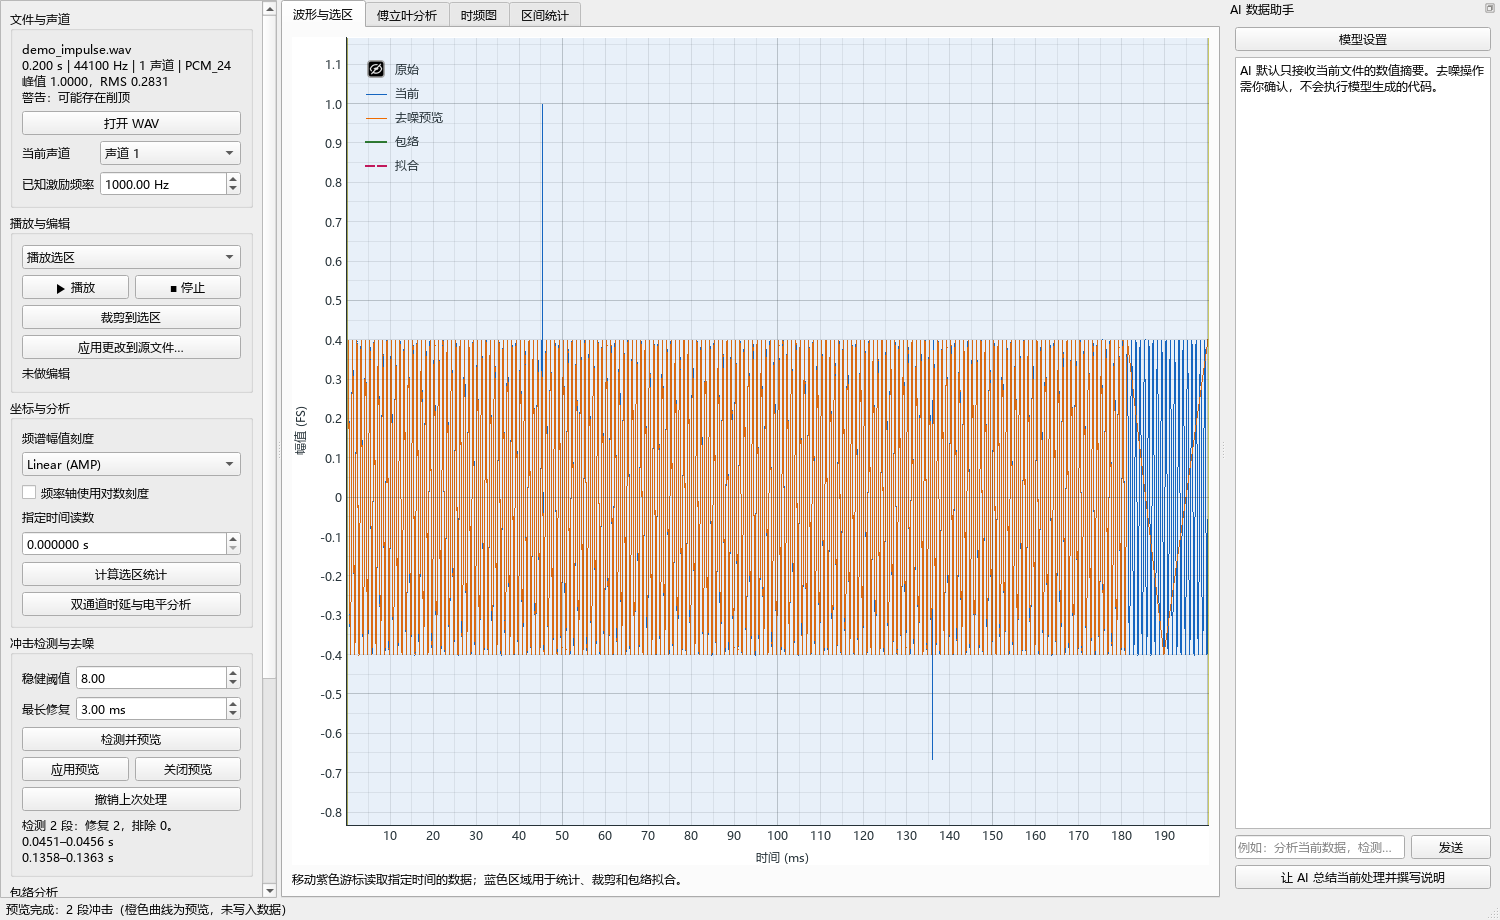
\includegraphics[width=0.96\textwidth]{01_waveform_denoise.png}
\caption{程序主界面（波形与选区页，含去噪预览）。左侧为控制区，中央为图表面板，右侧为 AI 数据助手。}
\label{fig:waveform}
\end{figure}

\begin{table}[htbp]
\centering
\caption{界面三区功能划分}
\begin{tabular}{@{}>{\raggedright\arraybackslash}p{2.4cm}>{\raggedright\arraybackslash}p{11.6cm}@{}}
\toprule
区域 & 主要功能 \\
\midrule
左侧控制区 & 打开文件、选择声道、设置频率、去噪、包络、统计、导出和批量处理 \\
中央图表面板 & 波形与选区、傅立叶分析、时频图、区间统计四个页签 \\
右侧 AI 助手 & 模型设置、会话输入、AI 分析与报告说明 \\
\bottomrule
\end{tabular}
\end{table}

\subsection{常用控件}

左侧控制区按功能分组，主要控件如下：

\begin{itemize}
  \item \textbf{打开 WAV}：选择需要分析的录音文件。
  \item \textbf{当前声道}：双通道文件可分别查看声道 1 与声道 2，不会自动混音。
  \item \textbf{已知激励频率}：输入实验实际使用的频率；不确定时可设为 0，由程序自动估计。
  \item \textbf{频谱幅值刻度}：在 Linear (AMP) 与 dBFS 之间切换。
  \item \textbf{频率轴对数刻度}：用于观察低频或跨多个数量级的频谱特征。
  \item \textbf{指定时间读数}：输入时间后，紫色游标移动到对应位置并显示局部幅值和频率信息。
  \item \textbf{蓝色选区}：拖动波形图上的蓝色区域，用于区间统计和包络拟合。
\end{itemize}

中央图表面板顶部有四个页签：“波形与选区”“傅立叶分析”“时频图”“区间统计”。切换页签不会改变已载入的数据和分析结果。

% ==================== 第 4 章 ====================
\section{数据导入与文件管理}

\subsection{支持格式与载入流程}

程序支持标准 PCM WAV 文件，包括单声道与双声道，常见位深如 16 bit、24 bit、32 bit float 均可读取。点击“打开 WAV”后选择文件，程序执行以下操作：读取采样数据、计算质量报告、初始化处理版本与有效掩码、清空历史撤销栈、重置 AI 会话，最后刷新全部图表。

载入成功后，左侧文件信息区显示文件名、时长、采样率、声道数、采样格式、峰值与 RMS。若检测到峰值接近满幅，会显示“警告：可能存在削顶”。削顶意味着信号被截断，频谱会出现额外谐波，应重新调整录音增益后重测。

\subsection{声道选择}

对于双通道文件，“当前声道”下拉框提供“声道 1”和“声道 2”。默认约定为：左声道（声道 1）是箱内参考，右声道（声道 2）是箱外接收。切换声道仅改变当前查看和分析的数据，不影响原始文件中的另一声道。所有去噪、包络、统计操作都只作用于当前声道的处理版本。

\subsection{只读原则与处理版本}

程序在内存中维护三份数据：原始样本（只读）、处理样本（可修改）、有效掩码（标记无效区间）。载入时处理样本与原始样本相同，有效掩码全为有效。每次应用去噪前，程序把当前处理样本和有效掩码压入撤销栈，因此可以随时回退。导出时输出的是处理版本，默认不会写回原始 WAV；确需写回时走“应用更改到源文件…”，程序先在同目录生成带时间戳的备份。撤销栈最多保留 4 级、合计约 1.2\,GB，超出后最早的记录被丢弃。

% ==================== 第 5 章 ====================
\section{波形显示与坐标读数}

\subsection{波形图元素}

“波形与选区”页如图~\ref{fig:waveform} 所示，横轴为时间（单位 s），纵轴为数字满幅归一化幅值（单位 FS）。波形图中的曲线含义如下：

\begin{itemize}
  \item \textbf{灰色曲线}：原始波形。仅当处理版本与原始版本不同时显示，便于对照。
  \item \textbf{蓝色曲线}：当前处理版本的波形。
  \item \textbf{橙色曲线}：去噪预览曲线。点击“检测并预览”后出现，确认前不会写入处理版本。
  \item \textbf{绿色曲线}：Hilbert 包络。
  \item \textbf{粉色虚线}：包络拟合曲线。
  \item \textbf{蓝色半透明选区}：当前统计与包络拟合的区间。
  \item \textbf{紫色竖线}：时间游标。
\end{itemize}

\subsection{蓝色选区}

波形图上的蓝色半透明区域表示当前选区。选区默认覆盖整个文件。拖动选区边界可以调整起点和终点。选区用于两项操作：点击“计算选区统计”时只统计选区内的数据；点击“显示包络并拟合选区”时只在选区内拟合包络模型。选区外的信号不会被这两项操作使用，但会完整参与傅立叶分析和时频图绘制。

\subsection{指定时间读数}

有两种方式读取指定时刻的数据：一是直接拖动紫色游标；二是在左侧“指定时间读数”输入框中输入时间值，游标会自动移动到该位置。读数结果\footnote{读数内容包括当前时刻的局部幅值、频率等信息，具体字段以程序显示为准。}显示在波形图下方的提示栏中。输入框支持 6 位小数，适合精确定位冲击发生时刻。

\subsection{幅值刻度与频率轴刻度}

左侧“频谱幅值刻度”下拉框提供两种选择：Linear (AMP) 显示单边幅值谱的线性幅值，dBFS 显示对应的分贝值。dBFS 定义为 $20\log_{10}(A/A_{\text{FS}})$，其中 $A_{\text{FS}}$ 为数字满幅。由于程序对窗函数进行了相干增益校正，谱峰幅值可以直接与原始信号的峰值振幅比较。

“频率轴使用对数刻度”复选框用于切换频谱图和相位图的横轴。分析低频现象或比较跨数量级的频率成分时，对数坐标更直观；观察高频谐波分布时，线性坐标更清晰。

% ==================== 第 6 章 ====================
\section{傅立叶分析}

\subsection{基本原理}

傅立叶分析把时域信号分解为不同频率的正弦分量。程序对当前声道的整个处理版本加窗后执行快速傅立叶变换（FFT），加窗目的是减少频谱泄漏。单边幅值谱经过窗函数相干增益校正，因此谱峰高度对应真实正弦分量的峰值振幅。

\subsection{结果页面}

“傅立叶分析”页如图~\ref{fig:fourier} 所示，上半部分为幅值谱和相位谱，下半部分为主要谱峰表和谐波表。

\begin{figure}[htbp]
\centering
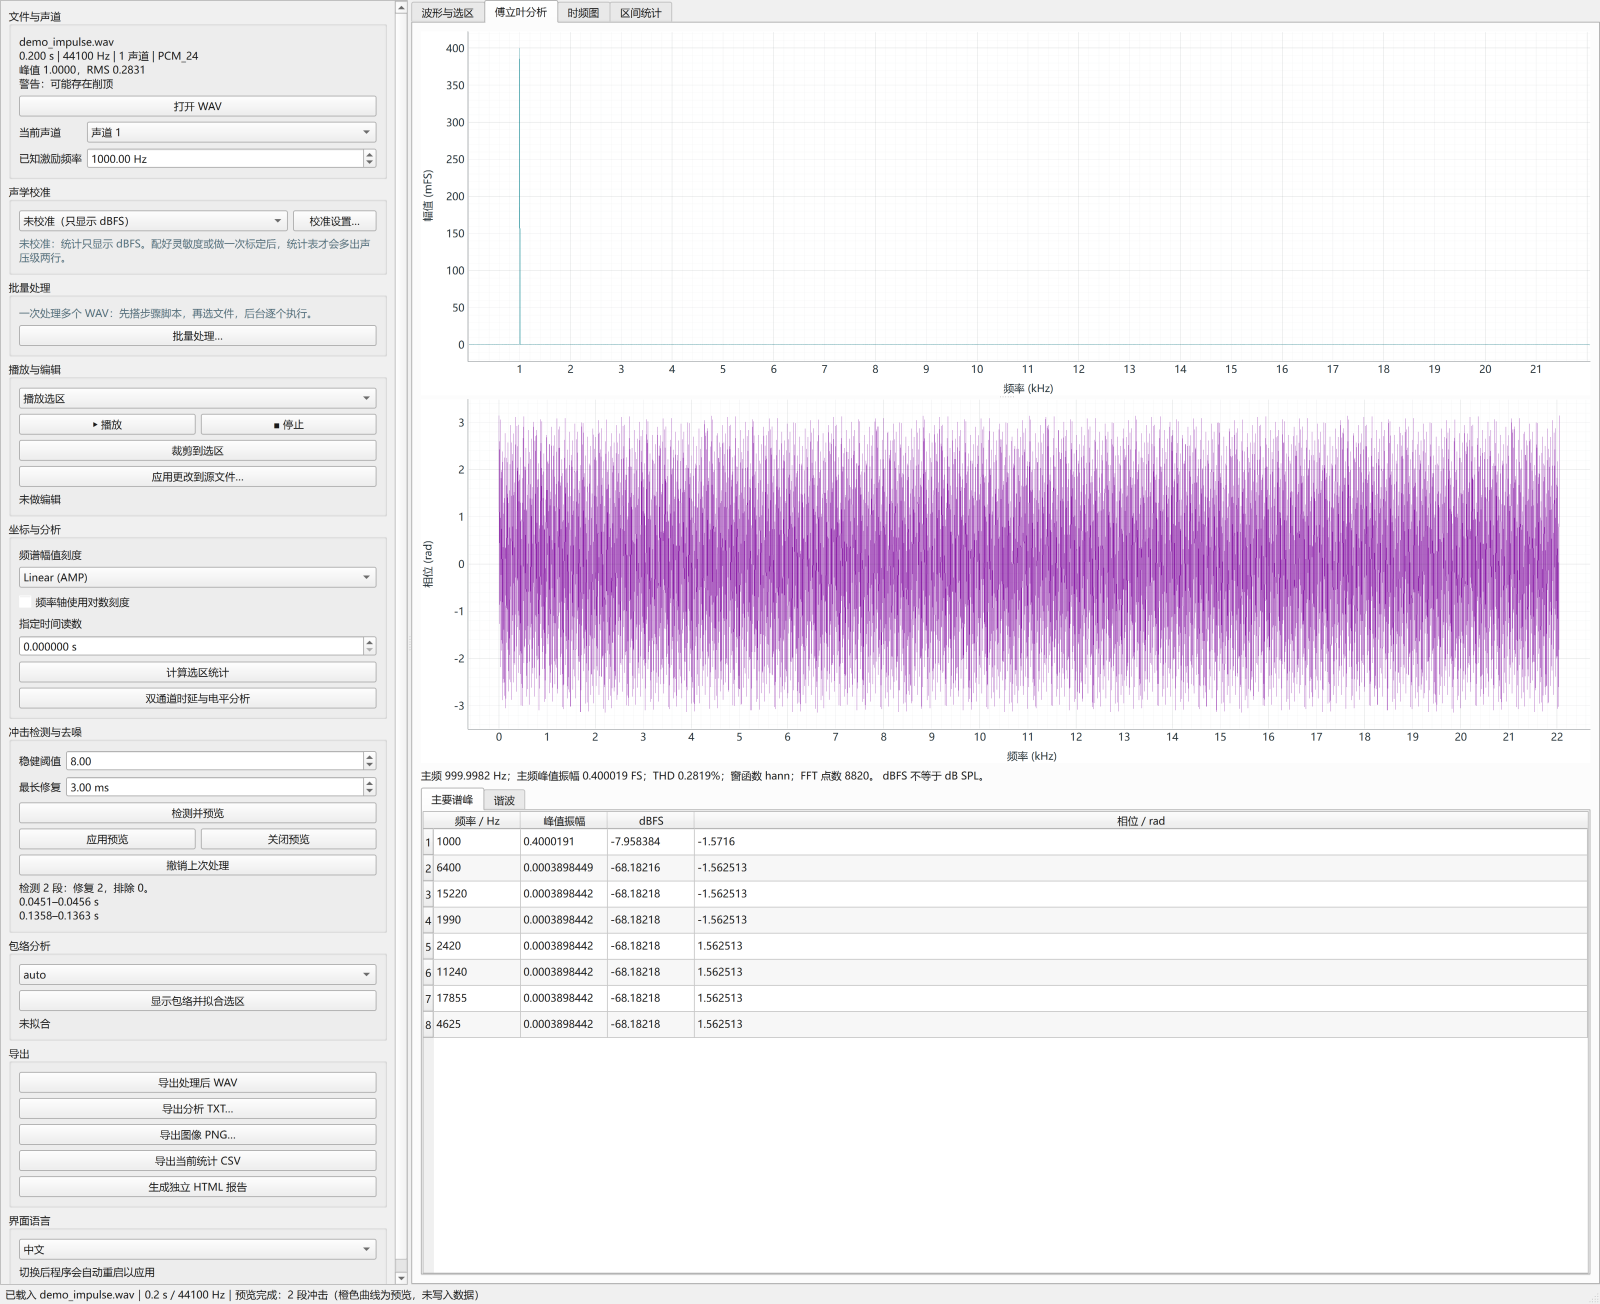
\includegraphics[width=0.96\textwidth]{02_fourier.png}
\caption{傅立叶分析页：上方为幅值谱与相位谱，下方为主要谱峰表与谐波表。}
\label{fig:fourier}
\end{figure}

摘要栏显示以下信息：

\begin{itemize}
  \item \textbf{主频}：幅度最大的频率分量。若“已知激励频率”设为 0，程序自动估计主频；若设为具体值，程序在该频率附近寻找峰值。
  \item \textbf{主频峰值振幅}：主频对应的峰值幅值，单位 FS。
  \item \textbf{THD}：总谐波失真，定义为各次谐波能量之和与基波能量之比。
  \item \textbf{窗函数与 FFT 点数}：当前使用的窗类型和变换点数。
\end{itemize}

主要谱峰表列出显著谱峰的频率、峰值振幅、dBFS 与相位。谐波表列出 1 至 8 次谐波的对应数值，便于观察开孔结构是否引入非线性失真。

\subsection{读数注意事项}

频谱图中的谱峰高度受信号时长、窗函数和频率分辨率影响。若信号过短，频率分辨率不足，相邻谱峰可能合并。若信号存在削顶，即使输入为纯正弦，频谱也会出现奇次谐波。此时应先检查波形是否存在平顶，再判断谐波是否来自开孔结构。

% ==================== 第 7 章 ====================
\section{时频分析}

\subsection{时频图的作用}

“时频图”页如图~\ref{fig:spectrogram} 所示，横轴为时间，纵轴为频率，颜色表示对应时刻和频率的能量强度。程序使用短时傅立叶变换（STFT）计算，颜色映射采用 viridis 色表。

\begin{figure}[htbp]
\centering
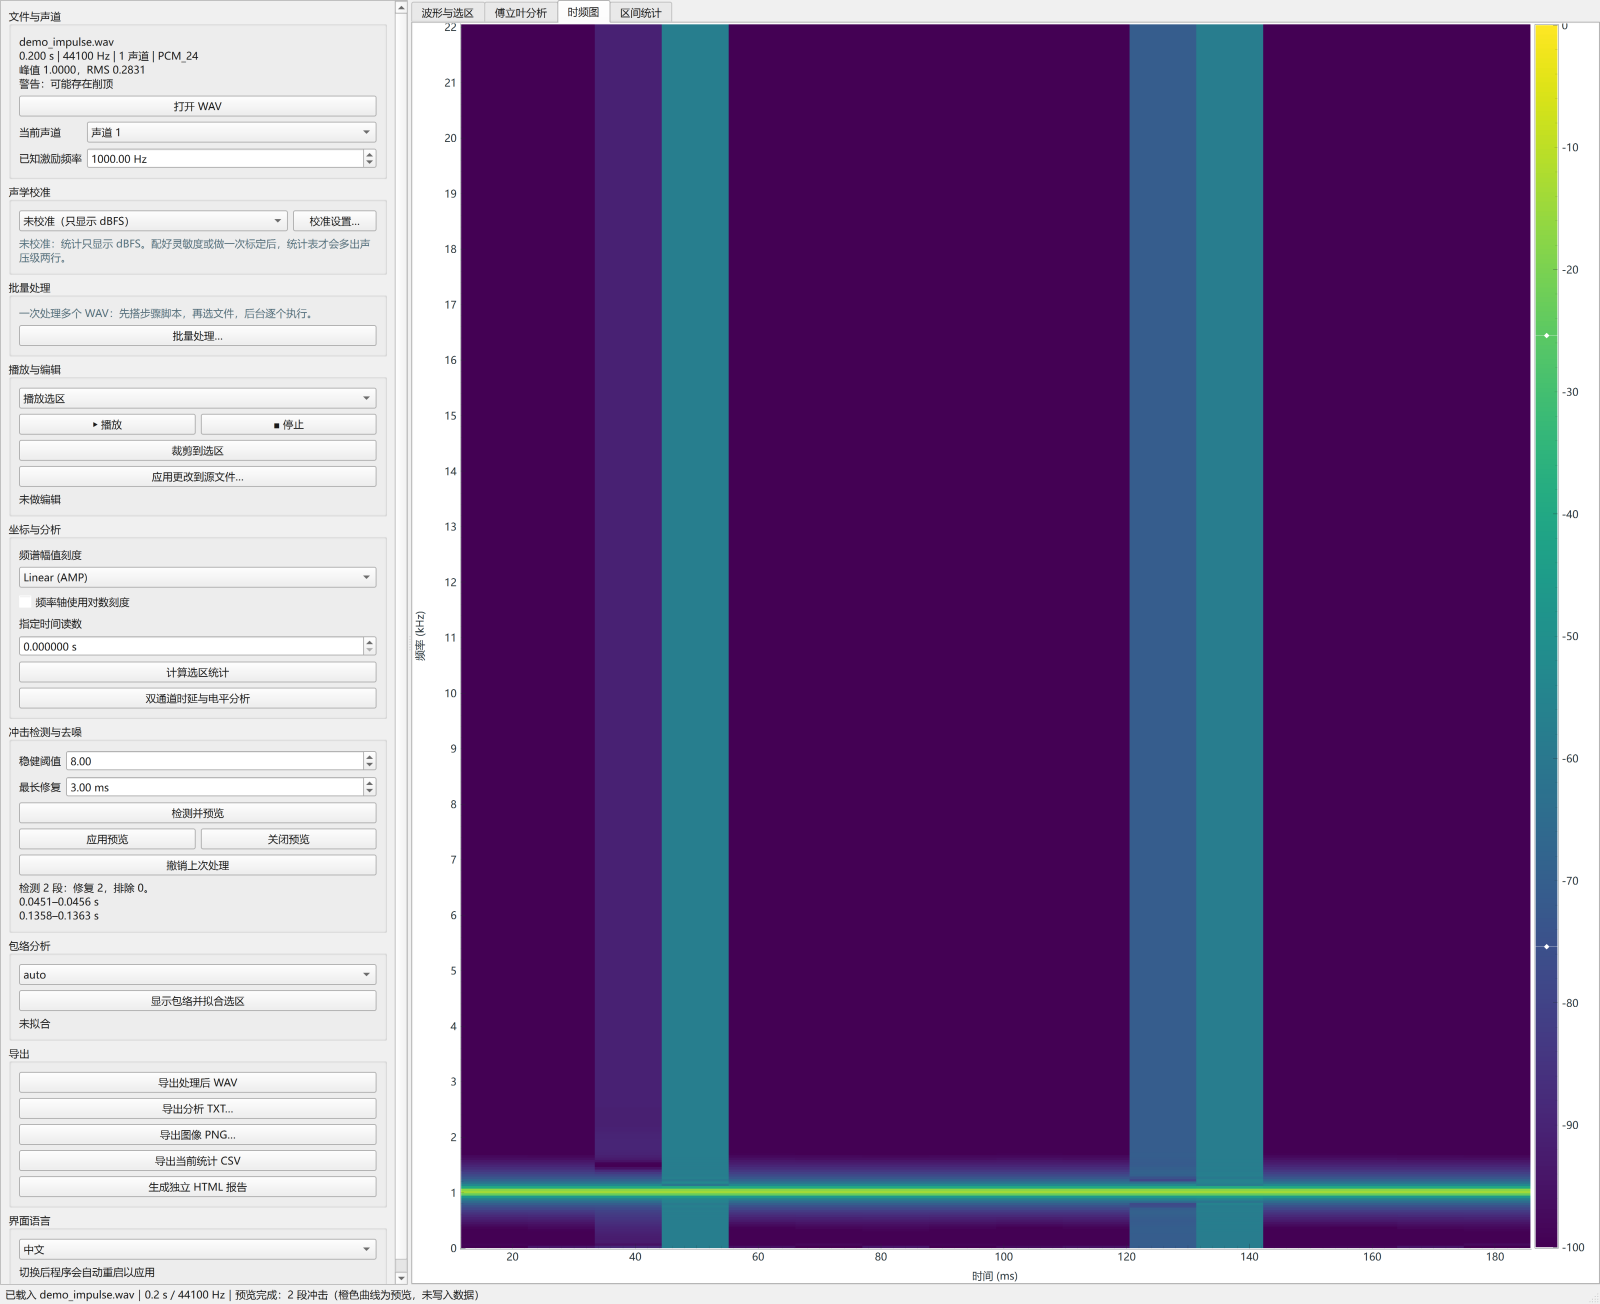
\includegraphics[width=0.96\textwidth]{03_spectrogram.png}
\caption{时频图页：持续正弦表现为水平亮带，冲击表现为短时竖直宽带。}
\label{fig:spectrogram}
\end{figure}

\subsection{典型特征解读}

持续稳定的正弦信号在时频图上表现为一条水平亮带，其纵坐标即为信号频率。冲击信号表现为短时、跨越宽频带的竖直亮条，与波形中的尖峰一一对应。若存在幅度突变（如 AGC 起效），时频图上会看到亮带强度突然变化。

时频图的主要用途是辅助判断冲击检测是否合理：先观察波形中的尖峰位置，再到时频图确认是否为宽带冲击，最后对照去噪预览中的修复区间。三者一致时，去噪结果才可信。

% ==================== 第 8 章 ====================
\section{冲击检测与去噪}

\subsection{冲击信号的来源与影响}

冲击信号可能来自样品放置时的碰撞、环境中突发敲击、电路干扰或数据采集瞬态。这类信号在时域上表现为孤立尖峰，在频域上会向全频段散布能量，显著抬高高次谐波和噪声底，影响 RMS、峰值因子和 THD 等统计量的准确性。

\subsection{检测算法}

程序采用稳健阈值检测：先计算信号的一阶差分和中值滤波残差，再用中位数绝对偏差估计稳健尺度，最后把超过阈值若干倍的采样点标记为冲击候选。使用稳健尺度而不是标准差，是为了避免冲击本身把阈值抬高，导致漏检。

左侧“冲击检测与去噪”分组提供两个参数：

\begin{itemize}
  \item \textbf{稳健阈值}：默认 8.0。数值越大，检出越少；数值越小，对异常越敏感。
  \item \textbf{最长修复}：默认 3.0 ms。只有短于该长度的冲击才会被插值修复。
\end{itemize}

\subsection{操作流程}

\begin{enumerate}
  \item 在左侧调整“稳健阈值”和“最长修复”。
  \item 点击“检测并预览”。
  \item 检查橙色预览曲线和事件位置列表，同时对照波形图与时频图。
  \item 若判定本次预览不合适（阈值不对、误标记太多），点击\textbf{“关闭预览”}把它丢弃：橙色曲线和待应用结果一并清除，处理版本与原文件都不受任何影响，改完参数可以重新检测。
  \item 确认无误后点击“应用预览”，预览结果才写入处理版本。
  \item 如需恢复，点击“撤销上次处理”。撤销最多保留最近 4 级，且总占用不超过约 1.2 GB，超出后自动丢弃最早的一级。
\end{enumerate}

“检测并预览”“应用预览”“关闭预览”三者的关系是：\textbf{检测只产生预览，预览可以随时关闭，只有“应用预览”才改动数据}。因此可以放心用不同阈值反复预览比较，不必担心污染实验数据。

\subsection{修复与排除策略}

程序按事件长度选择处理方式：短于“最长修复”的冲击用周围采样插值修复，尽量保持原始波形形态；长于该阈值或连续成片的冲击不凭空补造信号，而是标记为无效区间，在统计计算中自动排除。这一策略避免了用算法“编造”不存在的声学数据，保证实验结论的可信度。

应用去噪后，左侧标签显示检测到的事件数量、修复数量与排除数量，并列出前若干段事件的起止时间。状态栏提示“已应用到处理版本；原始 WAV 未修改”。

\subsection{人工复核要点}

自动阈值已通过合成信号验证，但真实实验数据可能包含不同类型的敲击、削顶和电磁干扰，自动结果必须人工复核。复核时重点检查：正常波峰是否被误标记、冲击起点和终点是否准确、排除区间是否覆盖了有效信号。若误标记频繁，应提高阈值、缩短最长修复，并检查数据是否削顶或存在直流偏置。

% ==================== 第 9 章 ====================
\section{播放与编辑}

\subsection{播放选区或全文件}

左侧“播放与编辑”分组用于试听，避免为听一段波形而切换软件。

\begin{itemize}
  \item \textbf{播放目标}：下拉框可选“播放选区”或“播放全文件”。选“播放选区”时只播放蓝色选区内的时间段。
  \item \textbf{播放与暂停}：同一个按钮在“播放”与“暂停”之间切换，暂停不丢失当前位置。
  \item \textbf{自动停止}：切换播放目标、载入新文件或关闭窗口时，播放自动停止并释放音频设备。
\end{itemize}

播放只读取处理版本用于监听，不改动任何数据，也不进入撤销栈。若声卡不支持文件采样率（例如 48\,kHz 文件在仅支持 44.1\,kHz 的设备上播放），程序会自动重采样后播放；该重采样只影响监听，不参与任何分析计算与导出。没有可用输出设备时，程序提示“当前系统没有可用的音频输出设备”，其余功能不受影响。

\subsection{裁剪到选区}

“裁剪到选区”把蓝色选区之外的数据丢弃，只保留选区内片段：

\begin{enumerate}
  \item 在波形图上框选要保留的区间。若选区已覆盖整个文件，程序提示“当前选区已覆盖整个文件”且不做任何改动。
  \item 点击“裁剪到选区”，处理样本、有效掩码与参考波形按同一区间同步截取。
  \item 状态栏回报保留的起止时间与采样点数，时间轴归零重新开始。
\end{enumerate}

裁剪前的状态会压入撤销栈，可随时用“撤销上次处理”还原。裁剪的两种常见用法：一是长录音只关心某一段响应，先裁剪再做统计与包络拟合，可显著减少后续计算量；二是先裁掉首尾的噪声段，让区间统计只覆盖有效信号。

\subsection{应用更改到源文件}

默认情况下所有编辑只作用于内存中的处理版本，原始 WAV 保持不变。若确实需要把处理结果落到原文件，点击“应用更改到源文件…”，程序按以下顺序执行：

\begin{enumerate}
  \item 把当前源文件复制为同目录下的 \texttt{.bak-时间戳.wav} 备份；
  \item 把处理版本按原始采样格式写回源文件路径；
  \item 清空撤销栈，编辑计数归零，参考波形更新为写回后的数据。
\end{enumerate}

写回不可撤销：撤销栈随之清空，唯一的恢复手段是那份备份文件（把备份改名回原文件名即可还原）。因此推荐顺序是先“导出处理后 WAV”确认结果无问题，再决定是否写回源文件。文件被播放器、网盘同步或杀毒软件占用时，写回会提示 \texttt{PermissionError}，关闭占用程序后重试即可。

\subsection{编辑状态与撤销栈}

编辑标签会显示“已应用 N 次编辑（去噪/裁剪），当前长度 X s；可写回源文件或撤销（可撤销 K 级）”，用于随时确认当前数据改了几次、还能退回几步。撤销栈最多保留 4 级、合计约 1.2\,GB；大文件连续多次编辑时最早的记录会被自动丢弃，以避免内存耗尽。需要长期保留中间结果时，请导出处理后的 WAV，而不是依赖撤销栈。

% ==================== 第 10 章 ====================
\section{包络分析}

\subsection{包络提取原理}

程序使用 Hilbert 变换提取解析信号，其模值即为瞬时幅值包络。包络反映了信号振幅随时间的变化，适合分析衰减过程、起振过程和幅度调制现象。

\subsection{操作流程与模型选择}

先在波形图上框选需要分析的区间，再点击“显示包络并拟合选区”。左侧“包络分析”分组提供四种模型：

\begin{itemize}
  \item \texttt{auto}：自动选择，程序根据拟合优度在候选模型中挑选。
  \item \texttt{constant}：常数模型，适合稳态信号。
  \item \texttt{linear}：线性模型，适合缓慢上升或下降的幅度变化。
  \item \texttt{exponential}：指数模型，适合衰减过程。
\end{itemize}

\begin{figure}[htbp]
\centering
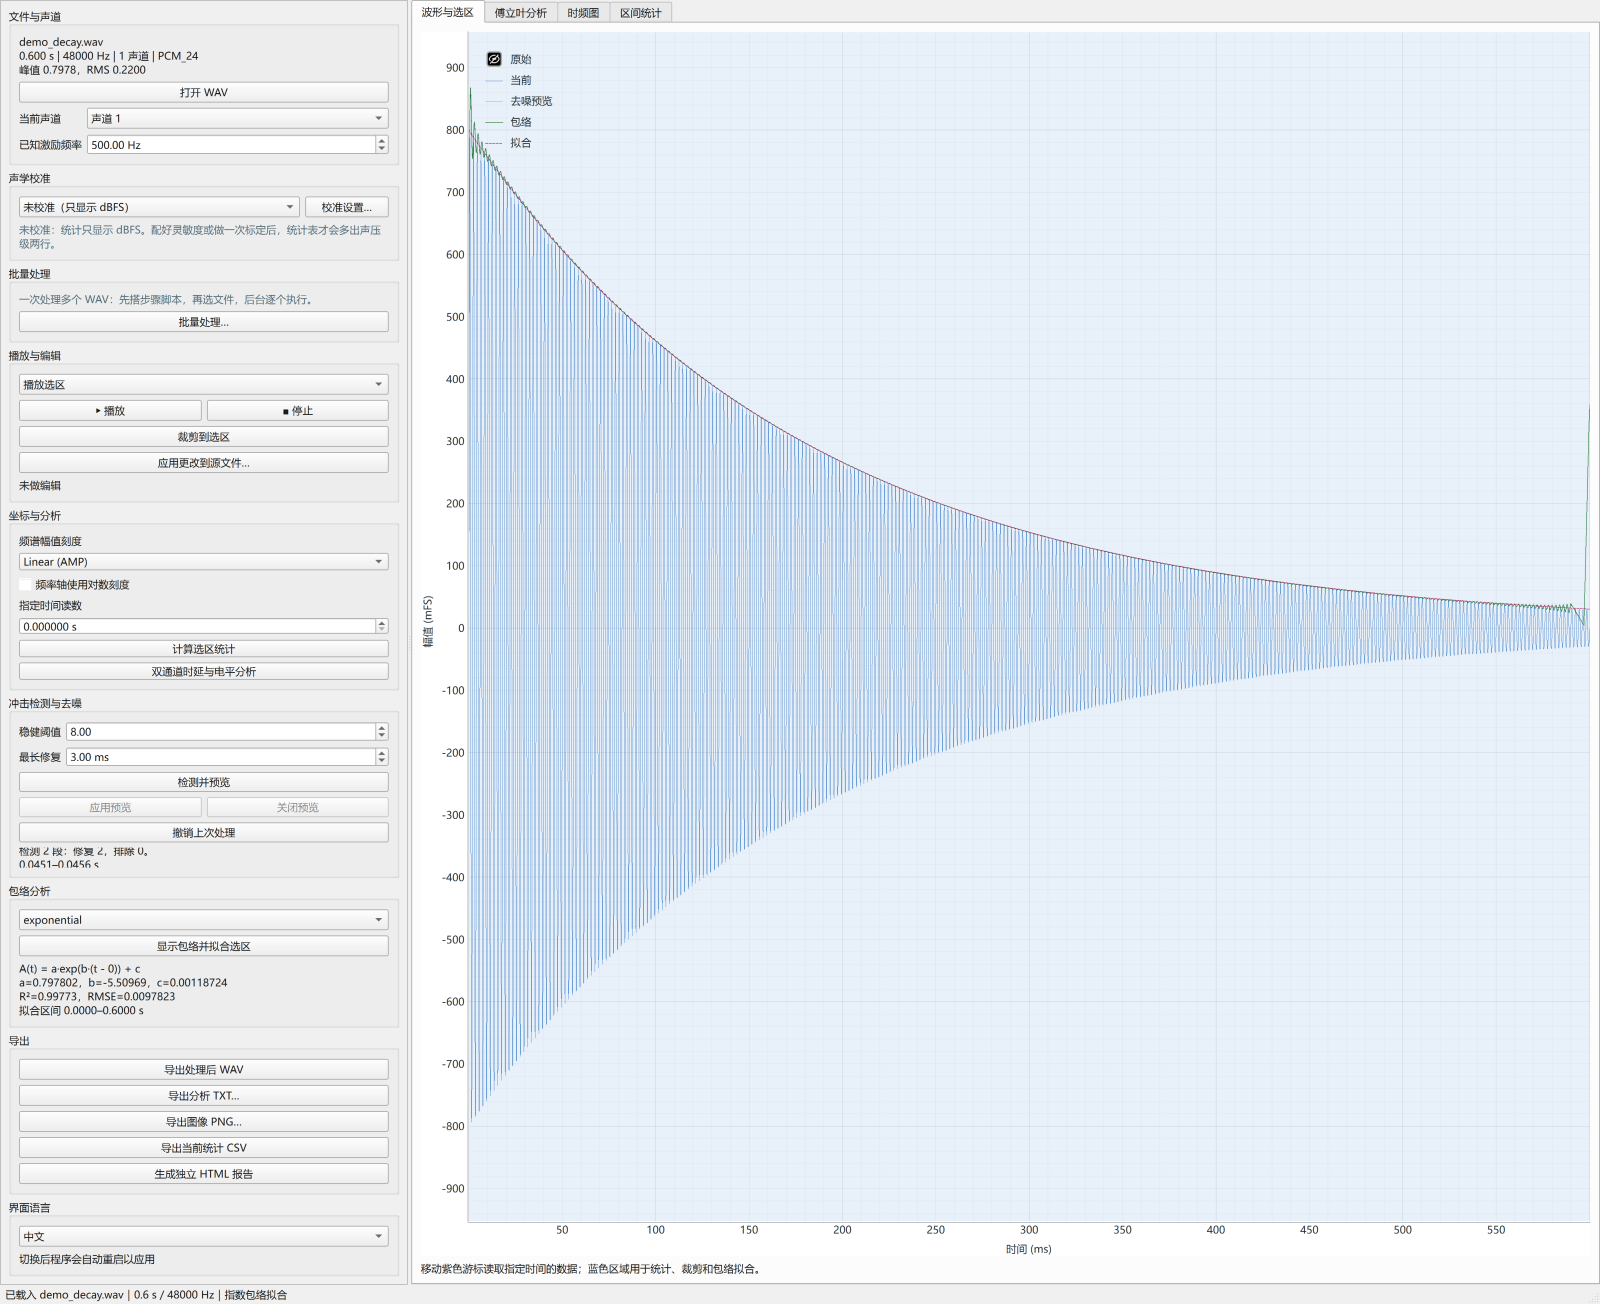
\includegraphics[width=0.96\textwidth]{05_envelope.png}
\caption{包络分析：绿色为 Hilbert 包络，粉色虚线为选区内的拟合曲线。}
\label{fig:envelope}
\end{figure}

如图~\ref{fig:envelope} 所示，拟合结果包括包络方程、参数值、决定系数 $R^2$ 和均方根误差 RMSE。稳态正弦通常接近常数包络；衰减过程可尝试指数模型。若 $R^2$ 很低或残差异常，应检查选区是否包含起止瞬态、冲击或 AGC 变化。

% ==================== 第 11 章 ====================
\section{区间统计}

\subsection{统计量说明}

“区间统计”页如图~\ref{fig:statistics} 所示。点击“计算选区统计”后，程序在当前蓝色选区内计算以下统计量：

\begin{figure}[htbp]
\centering
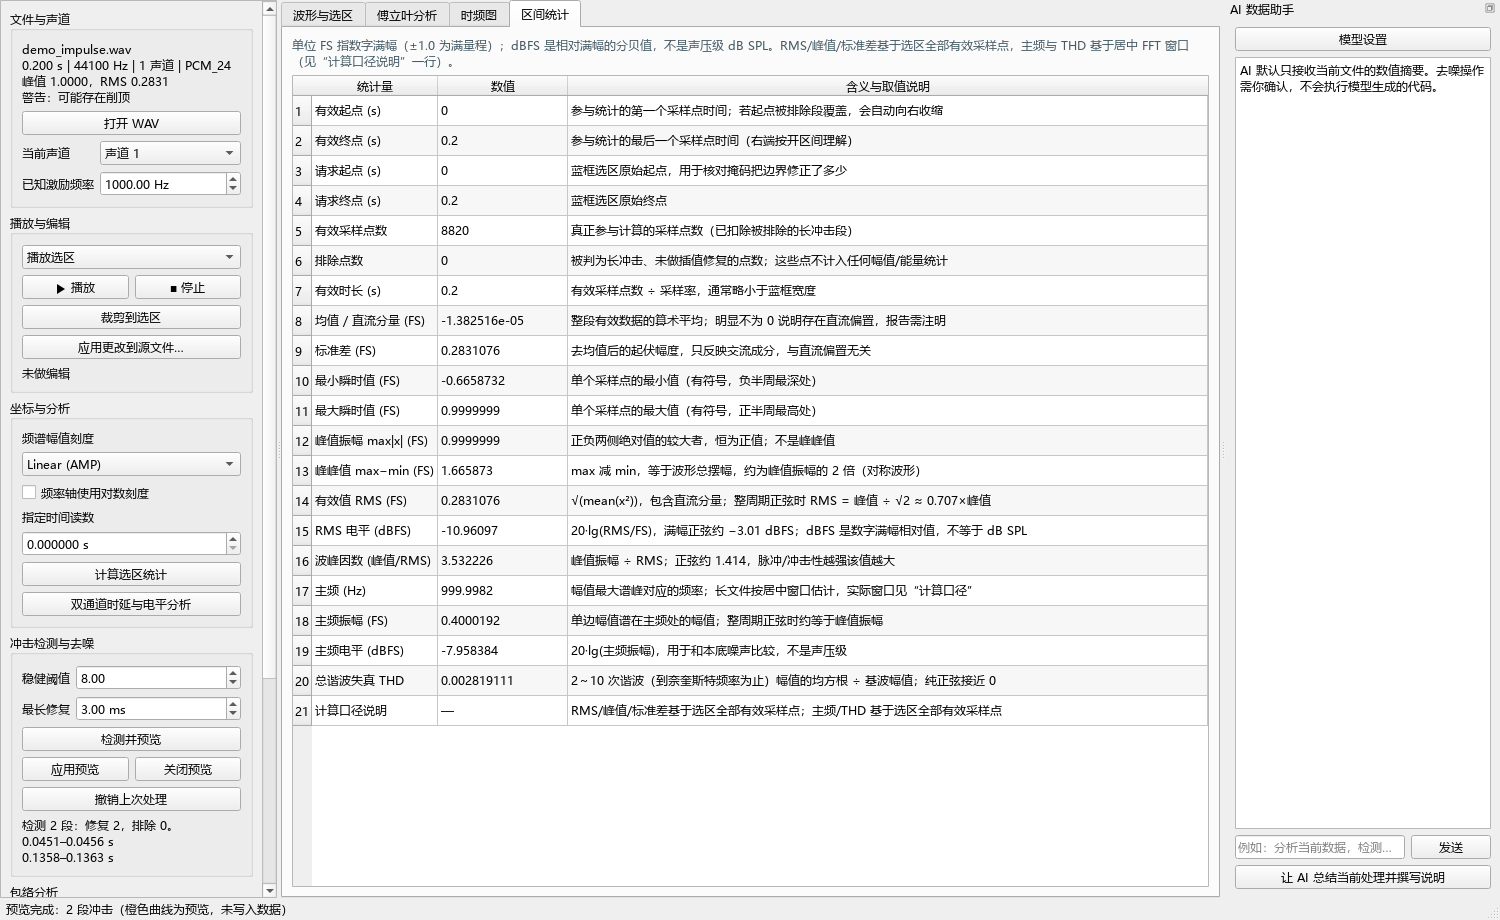
\includegraphics[width=0.96\textwidth]{04_statistics.png}
\caption{区间统计页：以表格形式显示选区内的统计量。}
\label{fig:statistics}
\end{figure}

程序的统计表用三列显示：\textbf{统计量（中文名）}、\textbf{数值}、\textbf{含义与取值说明}。只有中文名容易混淆的量（例如“峰值振幅”和“峰峰值”、“RMS”和“RMS 电平”），在第三列写清了区别，下表与程序界面逐行对应。

{\small
\begin{longtable}{@{}p{0.22\textwidth}p{0.26\textwidth}p{0.44\textwidth}@{}}
\caption{区间统计量释义（与程序“区间统计”页一一对应）}\\
\toprule
界面显示（中文名） & 对应键名 & 含义与取值说明 \\
\midrule
\endfirsthead
\toprule
界面显示（中文名） & 对应键名 & 含义与取值说明 \\
\midrule
\endhead
\bottomrule
\endfoot
有效起点 (s) & \texttt{start\_s} & 参与统计的第一个采样点时间；若起点被排除段覆盖，会自动向右收缩 \\
有效终点 (s) & \texttt{end\_s} & 参与统计的最后一个采样点时间（右端按开区间理解） \\
请求起点 (s) & \texttt{requested\_start\_s} & 蓝色选区的原始起点，用来核对掩码把边界修正了多少 \\
请求终点 (s) & \texttt{requested\_end\_s} & 蓝色选区的原始终点 \\
有效采样点数 & \texttt{samples} & 真正参与计算的采样点数，已扣除被排除的长冲击段 \\
排除点数 & \texttt{excluded\_samples} & 被判为长冲击、未做插值修复的点数，不进入任何幅值或能量统计 \\
有效时长 (s) & \texttt{duration\_s} & 有效采样点数 ÷ 采样率，通常略小于蓝色选区的宽度 \\
均值 / 直流分量 (FS) & \texttt{mean} & 有效数据的算术平均；明显不为 0 说明存在直流偏置，报告需注明 \\
标准差 (FS) & \texttt{std} & 去均值后的起伏幅度，只反映交流成分，与直流偏置无关 \\
最小瞬时值 (FS) & \texttt{min} & 单个采样点的最小值（有符号，负半周最深处） \\
最大瞬时值 (FS) & \texttt{max} & 单个采样点的最大值（有符号，正半周最高处） \\
峰值振幅 (FS) & \texttt{peak\_amplitude} & $\max|x|$，恒为正值；不是峰峰值，也不是 RMS \\
峰峰值 (FS) & \texttt{peak\_to\_peak} & $\max-\min$，波形总摆幅；对称波形约为峰值振幅的 2 倍 \\
有效值 RMS (FS) & \texttt{rms} & 均方根 $\sqrt{\mathrm{mean}(x^2)}$，含直流分量；整周期正弦时等于峰值 ÷ $\sqrt{2}$ \\
RMS 电平 (dBFS) & \texttt{rms\_dbfs} & $20\lg(\mathrm{RMS}/\mathrm{FS})$，满幅正弦约 $-3.01$ dBFS；dBFS 不是声压级 dB SPL \\
波峰因数 & \texttt{crest\_factor} & 峰值振幅 ÷ RMS；正弦约 1.414，脉冲或冲击性越强该值越大 \\
主频 (Hz) & \texttt{main\_frequency\_hz} & 幅值最大谱峰对应的频率；长文件按居中窗口估计，实际窗口见“计算口径说明” \\
主频振幅 (FS) & \texttt{main\_amplitude} & 单边幅值谱在主频处的幅值；整周期正弦时约等于峰值振幅 \\
主频电平 (dBFS) & \texttt{main\_amplitude\_dbfs} & $20\lg(\text{主频振幅})$，用于与本底噪声比较，不是声压级 \\
总谐波失真 THD & \texttt{thd} & 2～10 次谐波（到奈奎斯特频率为止）幅值的均方根 ÷ 基波幅值；纯正弦接近 0 \\
计算口径说明 & \texttt{analysis\_scope} & 声明哪些量基于选区全部采样点、哪些量基于受限 FFT 窗口 \\
\end{longtable}
}

导出 CSV 时使用第二列的键名，便于脚本批量处理；界面、HTML 报告与 AI 说明使用中文名。两者指的是同一个量。

\subsection{无效区间处理}

统计量会自动排除已标记为无效的长冲击区间。这意味着即使选区覆盖了整段录音，被排除区间的样本也不会进入计算。若需要统计特定稳态段，建议手动缩小蓝色选区，避免起止瞬态影响结果。

统计结果可通过左侧“导出当前统计 CSV”按钮保存为 CSV 文件，便于在 Excel 或 Python 中进一步处理。

\subsection{长音频处理与数值口径}

本程序面向的实验录音可能很长（例如十几分钟、数千万采样点）。为避免界面在分析超长文件时失去响应，程序对显示与频谱计算做了性能优化。理解各类数据的计算口径，对正确引用实验结果至关重要：

\begin{itemize}
  \item \textbf{能量类统计量}（RMS、峰值、峰峰值、均值、标准差、峰值因子）：始终基于所选区间的\textbf{全部有效采样点}计算，未做任何抽稀，精度不受影响。
  \item \textbf{主频与 THD}：为避免全量 FFT 造成长时间卡顿，默认基于居中的约 5.5 秒窗口（262,144 点）计算，频率分辨率约 \texttt{采样率/262144}（48 kHz 下约 0.18 Hz）。“傅立叶分析”页和状态栏会明确标注实际分析的时间范围与点数，程序不会在未告知的情况下只分析局部数据。若需更高频率分辨率（例如精密稳态标定），可在源码中调用 \texttt{fourier\_analysis(..., max\_samples=0)} 执行全量分析。
  \item \textbf{波形显示与时频图}：仅做可视化抽稀（波形按列保留极值、时频图跳帧），\textbf{不参与任何数值计算}，因此不影响统计结果。时频图的时间采样较稀，短时冲击建议以波形图为主要定位依据。
  \item \textbf{游标包络读数}：使用中心对称窗口求 Hilbert 包络并取中心值，避免边缘效应对稳态信号造成系统偏差。
\end{itemize}

在实验报告中引用主频、THD 等频谱量时，应同时记录程序标注的分析窗口与点数，以便结果可复核。

% ==================== 第 12 章 ====================
\section{声学校准}

\subsection{为什么需要校准}

程序内部一切幅值都是相对数字满幅的：FS 表示 $|x|$ 相对满幅的比例，dBFS 是 $20\lg|x|$。比较同一次录音内部的两段信号，这套相对单位完全够用；但实验报告里常要给出绝对声压级，那必须把读数挂到具体的麦克风上。

换算只需要一个加性常数。设麦克风灵敏度 $S$（V/Pa）、前置增益 $G$（线性倍数，$G=10^{G_\mathrm{dB}/20}$）、声卡 0\,dBFS 对应的输入电压 $V_\mathrm{fs}$，则

\begin{equation}
L_\mathrm{SPL} = L_\mathrm{dBFS} + K, \qquad
K = 20\lg\frac{V_\mathrm{fs}}{G\,S\,p_0}, \qquad p_0 = 20\ \mu\mathrm{Pa}.
\label{eq:calib}
\end{equation}

推导只有三步：输入电压 $V_\mathrm{adc} = V_\mathrm{fs}\cdot10^{L_\mathrm{dBFS}/20}$，声压 $p = V_\mathrm{adc}/(GS)$，再对 $p/p_0$ 取 20 倍对数。三处都是乘除，取对数后变成加减，所以整批数据共用同一个 $K$——校准一次，之后每加一行都是简单的加法。

以常见驻极体话筒为例：$S=10$\,mV/Pa、无前置增益、声卡满幅 1\,Vrms，代入得 $K=+133.98$\,dB。验算：94\,dB SPL 恰好对应 1\,Pa，麦克风输出 10\,mV，相对 1\,Vrms 是 $-40$\,dBFS，$-40+133.98=93.98$，与标称值只差 0.02\,dB（四舍五入造成）。

\subsection{两种输入方式}

左侧“声学校准”分组里点“校准设置…”，打开图~\ref{fig:calib_params} 的对话框。$K$ 有两条来路，二者等效：

\begin{figure}[H]
\centering
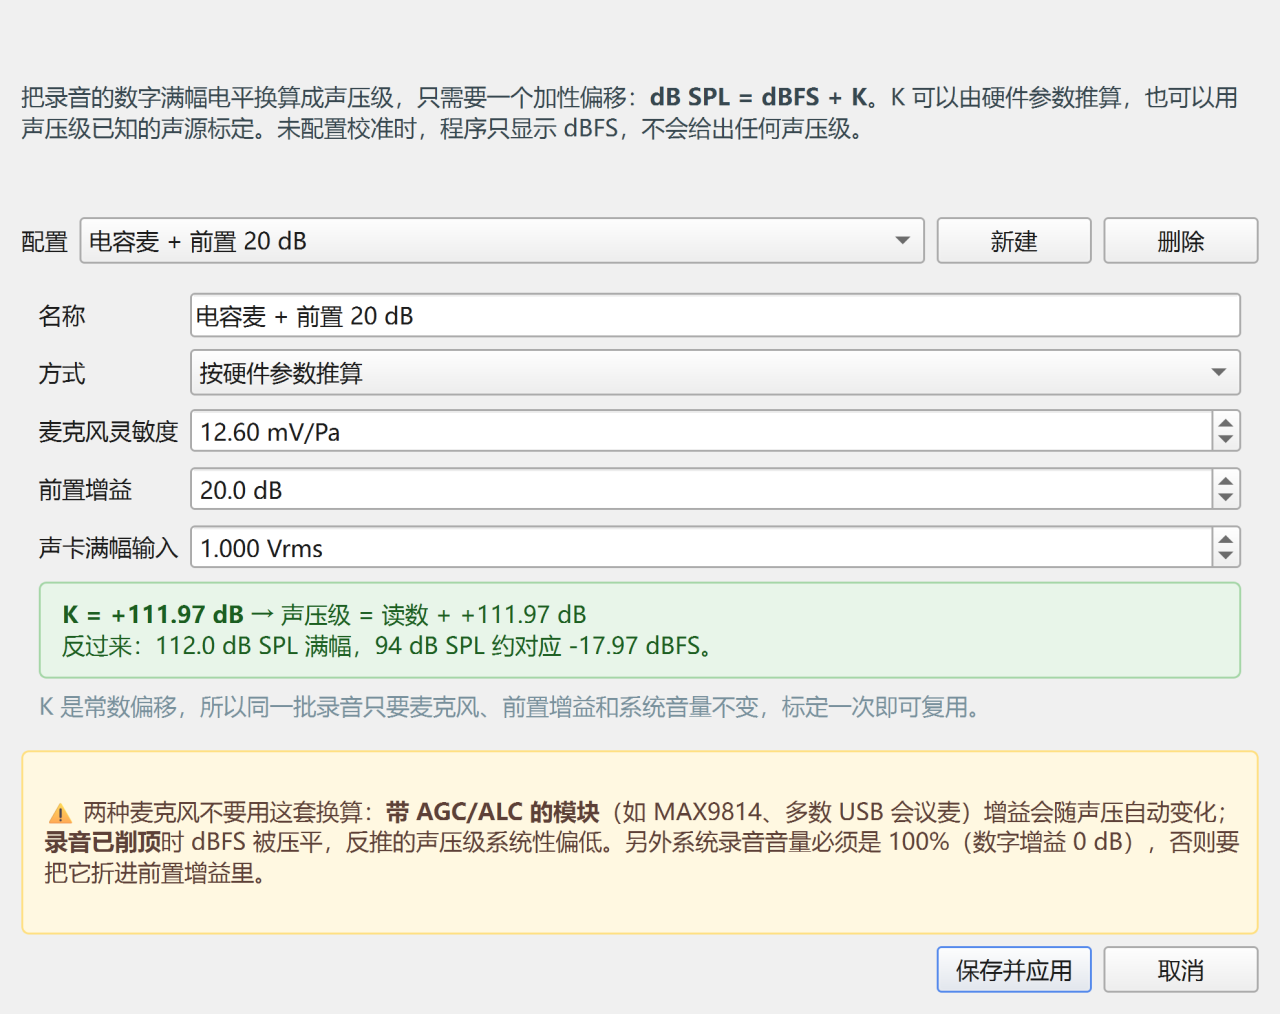
\includegraphics[width=0.84\textwidth]{13_calibration.png}
\caption{按硬件参数推算。绿色框实时给出 $K$，并反算出“94 dB SPL 大约对应多少 dBFS”，方便当场验算。}
\label{fig:calib_params}
\end{figure}

\begin{itemize}
  \item \textbf{按硬件参数推算}：填灵敏度、前置增益、声卡满幅输入电压。表~\ref{tab:calib_examples} 给出几种常见链路的 $K$，可用于核对填入的参数是否合理。
  \item \textbf{按已知声压级标定}：拿一个声压级已知的声源（声级校准器，或已标定过的手机播放固定音），填它标称的声压级与程序读到的 dBFS，$K=L_\mathrm{ref}-L_\mathrm{dBFS}$。这条路不需要知道 $V_\mathrm{fs}$——而 $V_\mathrm{fs}$ 恰恰是民用声卡最不可靠的参数。
\end{itemize}

\begin{table}[htbp]
\centering
\caption{几种常见链路的校准偏移（$V_\mathrm{fs}$ 取标称值，实际可能有偏差）}
{\small
\begin{tabular}{@{}>{\raggedright\arraybackslash}p{3.0cm}>{\raggedright\arraybackslash}p{2.4cm}>{\raggedright\arraybackslash}p{2.4cm}>{\raggedright\arraybackslash}p{1.9cm}>{\raggedright\arraybackslash}p{4.4cm}@{}}
\toprule
链路 & 灵敏度 & 前置增益 & $K$ / dB & 说明 \\
\midrule
驻极体 + 声卡 & 10 mV/Pa & 0 dB, 1 Vrms & 133.98 & 教科书基准 \\
同上 + 前置放大 & 10 mV/Pa & 20 dB, 1 Vrms & 113.98 & 增益每加 20 dB，$K$ 少 20 \\
高灵敏电容麦 & 50 mV/Pa & 0 dB, 1 Vrms & 120.00 & 灵敏度高 14 dB，$K$ 低 14 \\
专业声卡 & 12.6 mV/Pa & 20 dB, 0.775 Vrms & 109.76 & 满幅取 $-2.2$ dB，$K$ 再低一点 \\
\bottomrule
\end{tabular}}
\label{tab:calib_examples}
\end{table}

第二张图是标定方式（图~\ref{fig:calib_ref}）。点“取当前统计”会把当前选区的 RMS 电平直接填进“对应读数”，省得手抄；前提是先算过一次选区统计。

\begin{figure}[H]
\centering
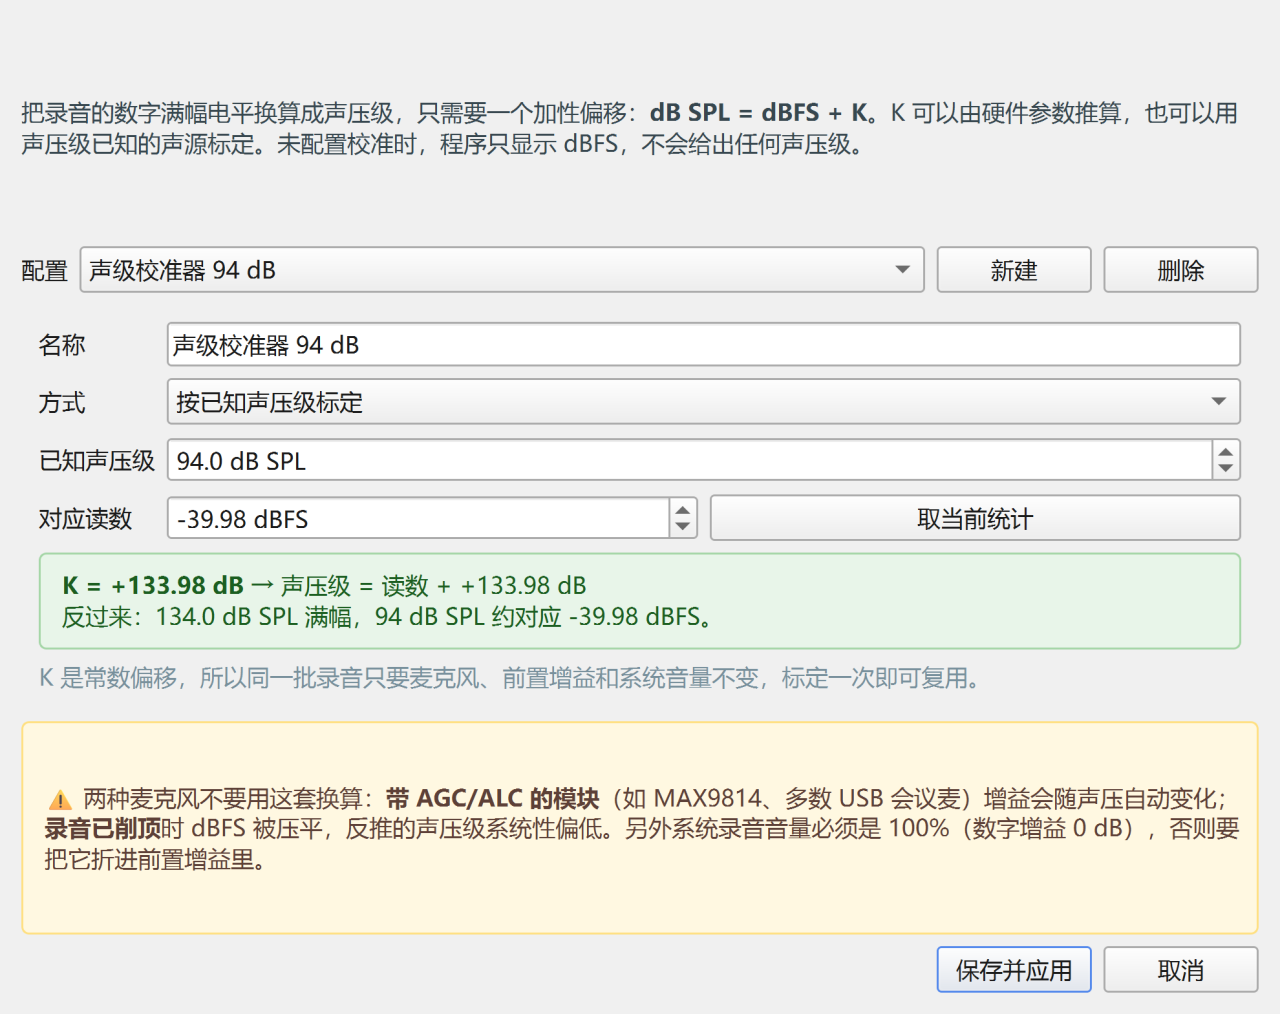
\includegraphics[width=0.84\textwidth]{14_calibration_ref.png}
\caption{按已知声压级标定。灵敏度与增益等参数此时隐藏，只留“已知声压级”与“对应读数”两行。}
\label{fig:calib_ref}
\end{figure}

\begin{quote}
\textbf{标定的正确做法}：把声源稳定地开到标称声压级（例如校准器套在麦克风上，94 dB SPL），录一段 3 秒以上；在程序里选中这段稳态区间、点“计算选区统计”，读出 RMS 电平；再到校准对话框选“按已知声压级标定”，点“取当前统计”。这条路的精度取决于声源本身是否可信，而不是声卡的参数。
\end{quote}

\subsection{校准如何影响结果}

校准配置保存在本机（与 AI 设置同一处配置存储），可保存多个、按名称切换。切换配置时，\textbf{已经算好的统计会就地重算声压级}，不重新做 FFT——统计量本身没变，变的只是一个加性偏移，所以切换是瞬时的。

几处输出的变化见表~\ref{tab:calib_outputs}。

\begin{table}[htbp]
\centering
\caption{配置校准后各处的变化}
{\small
\begin{tabular}{@{}>{\raggedright\arraybackslash}p{3.4cm}>{\raggedright\arraybackslash}p{10.4cm}@{}}
\toprule
位置 & 变化 \\
\midrule
区间统计表 & 新增“峰值声压级”与“等效声压级”两行，紧跟在对应的 dBFS 行之后；末尾两行给出 $K$ 与配置名 \\
统计 CSV & 多出 \texttt{peak\_spl}、\texttt{rms\_spl}、\texttt{calibration\_offset\_db} 三列，dBFS 列照旧保留 \\
分析 TXT & 文件头增加“声学校准”一行（配置名与 $K$），并附三行限定条件；区间统计段同步多出两行 \\
HTML 报告 & 统计表同步多出两行，页脚说明改为“按声学校准换算”，并注明未计频率计权 \\
批量处理 & 整批共用主界面当前选中的那一组校准；CSV 与 TXT 的合并输出同样带声压级 \\
\bottomrule
\end{tabular}}
\label{tab:calib_outputs}
\end{table}

\textbf{未配置校准时，程序不输出任何 dB SPL 字段}。这是有意的：填充一个看起来合理、实则没有标定依据的数字，比留空危险得多。

\needspace{9\baselineskip}
\subsection{什么情况下这个换算不成立}

\begin{enumerate}
  \item \textbf{带 AGC/ALC 的麦克风}（MAX9814 模块、多数 USB 会议麦）：增益随声压自动变化，$K$ 不是常数。这类设备只能做相对比较，不能给绝对声压级。
  \item \textbf{录音已削顶}：削顶后 dBFS 被压平在 0 附近，反推的声压级系统性偏低。先看质量检查里的削顶警告。
  \item \textbf{系统录音音量不是 100\%}：Windows 的输入音量是数字增益，等效于给 $G$ 多加一项。要么固定在 100\%，要么把这一项折进“前置增益”里一起填。
  \item \textbf{声卡满幅电压未知或标称值不准}：这是参数推算最大的不确定度来源。有条件就改用已知声压级标定。
  \item \textbf{需要频率计权的量}：程序给出的是不计权（Z 计权）的声压级，不是 dBA。要报 dBA 需在频域按 A 计权曲线加权后再积分。
\end{enumerate}

\subsection{一个完整的校准例子}

以本实验的隔音箱透射测量为例，链路是“驻极体话筒 $\to$ 前置放大 30 dB $\to$ USB 声卡（满幅 1 Vrms）”，话筒灵敏度标称 12.6 mV/Pa：

\begin{enumerate}
  \item 算 $K$：$K = 133.98 - 20\lg(12.6/10) - 30 = 133.98 - 2.01 - 30 = 101.97$\,dB。
  \item 在对话框里填 $S=12.6$、增益 30、满幅 1.0，确认绿框显示 $K=+101.97$\,dB。
  \item 保存为“驻极体 +30 dB”，之后每次打开程序自动沿用。
  \item 录一段已知声源（如 94 dB 校准器）复核：若程序读到 $-8.03$\,dBFS，则 $-8.03+101.97=93.94$，与标称值差 0.06\,dB，说明参数填得对。若差得多，改用标定方式直接用实测值定 $K$。
  \item 批量处理 145 个文件时，主界面选中的这组校准会整批生效，CSV 里直接得到各测点的等效声压级与峰值声压级，再做 $\Delta L$ 相减就是隔声量。
\end{enumerate}

\begin{quote}
\textbf{提醒}：$\Delta L$ 是两个声压级相减，$K$ 在相减时会抵消。所以只要整批用的是同一套硬件与增益，即使 $K$ 有 1\,dB 的偏差，隔声量仍然是准的。校准真正影响的是\textbf{绝对声压级}，以及跨不同增益批次的数据能否直接比较。
\end{quote}

% ==================== 第 13 章 ====================
\section{双通道分析}

\subsection{分析内容}

对于双通道文件，点击“双通道时延与电平分析”可弹出结果窗口，显示：

\begin{itemize}
  \item \textbf{互相关时延}：通过互相关函数峰值位置估计两路信号的时间差。
  \item \textbf{峰值质量}：互相关峰值的尖锐程度，反映估计的可信度。
  \item \textbf{两路 RMS 电平}：声道 1 与声道 2 的均方根电平。
  \item \textbf{电平差}：两路电平之差，常用于估算隔声效果。
\end{itemize}

\subsection{AGC 风险提示}

若录音设备使用 MAX9814 等带自动增益控制（AGC）的麦克风模块，麦克风增益会随声压变化自动调整，两路幅值比不再准确反映真实声压比。此时电平差不能直接视为隔声量。强度结论应结合声级计读数或可靠的幅值校准，且报告中必须注明 AGC 是否工作。

% ==================== 第 14 章 ====================
\section{AI 数据助手}

\subsection{模型配置}

点击右侧“模型设置”（图~\ref{fig:ai_settings}）。对话框顶部是\textbf{厂商预设}，选好厂商后 Base URL 与常用模型名会自动填好，你只需要填 API Key：

\begin{itemize}
  \item \textbf{DeepSeek（深度求索）}：\texttt{https://api.deepseek.com/v1}，模型 \texttt{deepseek-chat}、\texttt{deepseek-reasoner}。
  \item \textbf{Moonshot（月之暗面 Kimi）}：\texttt{https://api.moonshot.cn/v1}，模型 \texttt{kimi-latest}、\texttt{kimi-k2-0905-preview} 等。
  \item \textbf{OpenAI}：\texttt{https://api.openai.com/v1}，模型 \texttt{gpt-4.1-mini} 等。
  \item \textbf{自定义（自填 Base URL 与模型名）}：适用于学校或实验室自建网关、代理服务以及上述三家之外的兼容服务，三项都要自己填。
\end{itemize}

\begin{figure}[H]
\centering
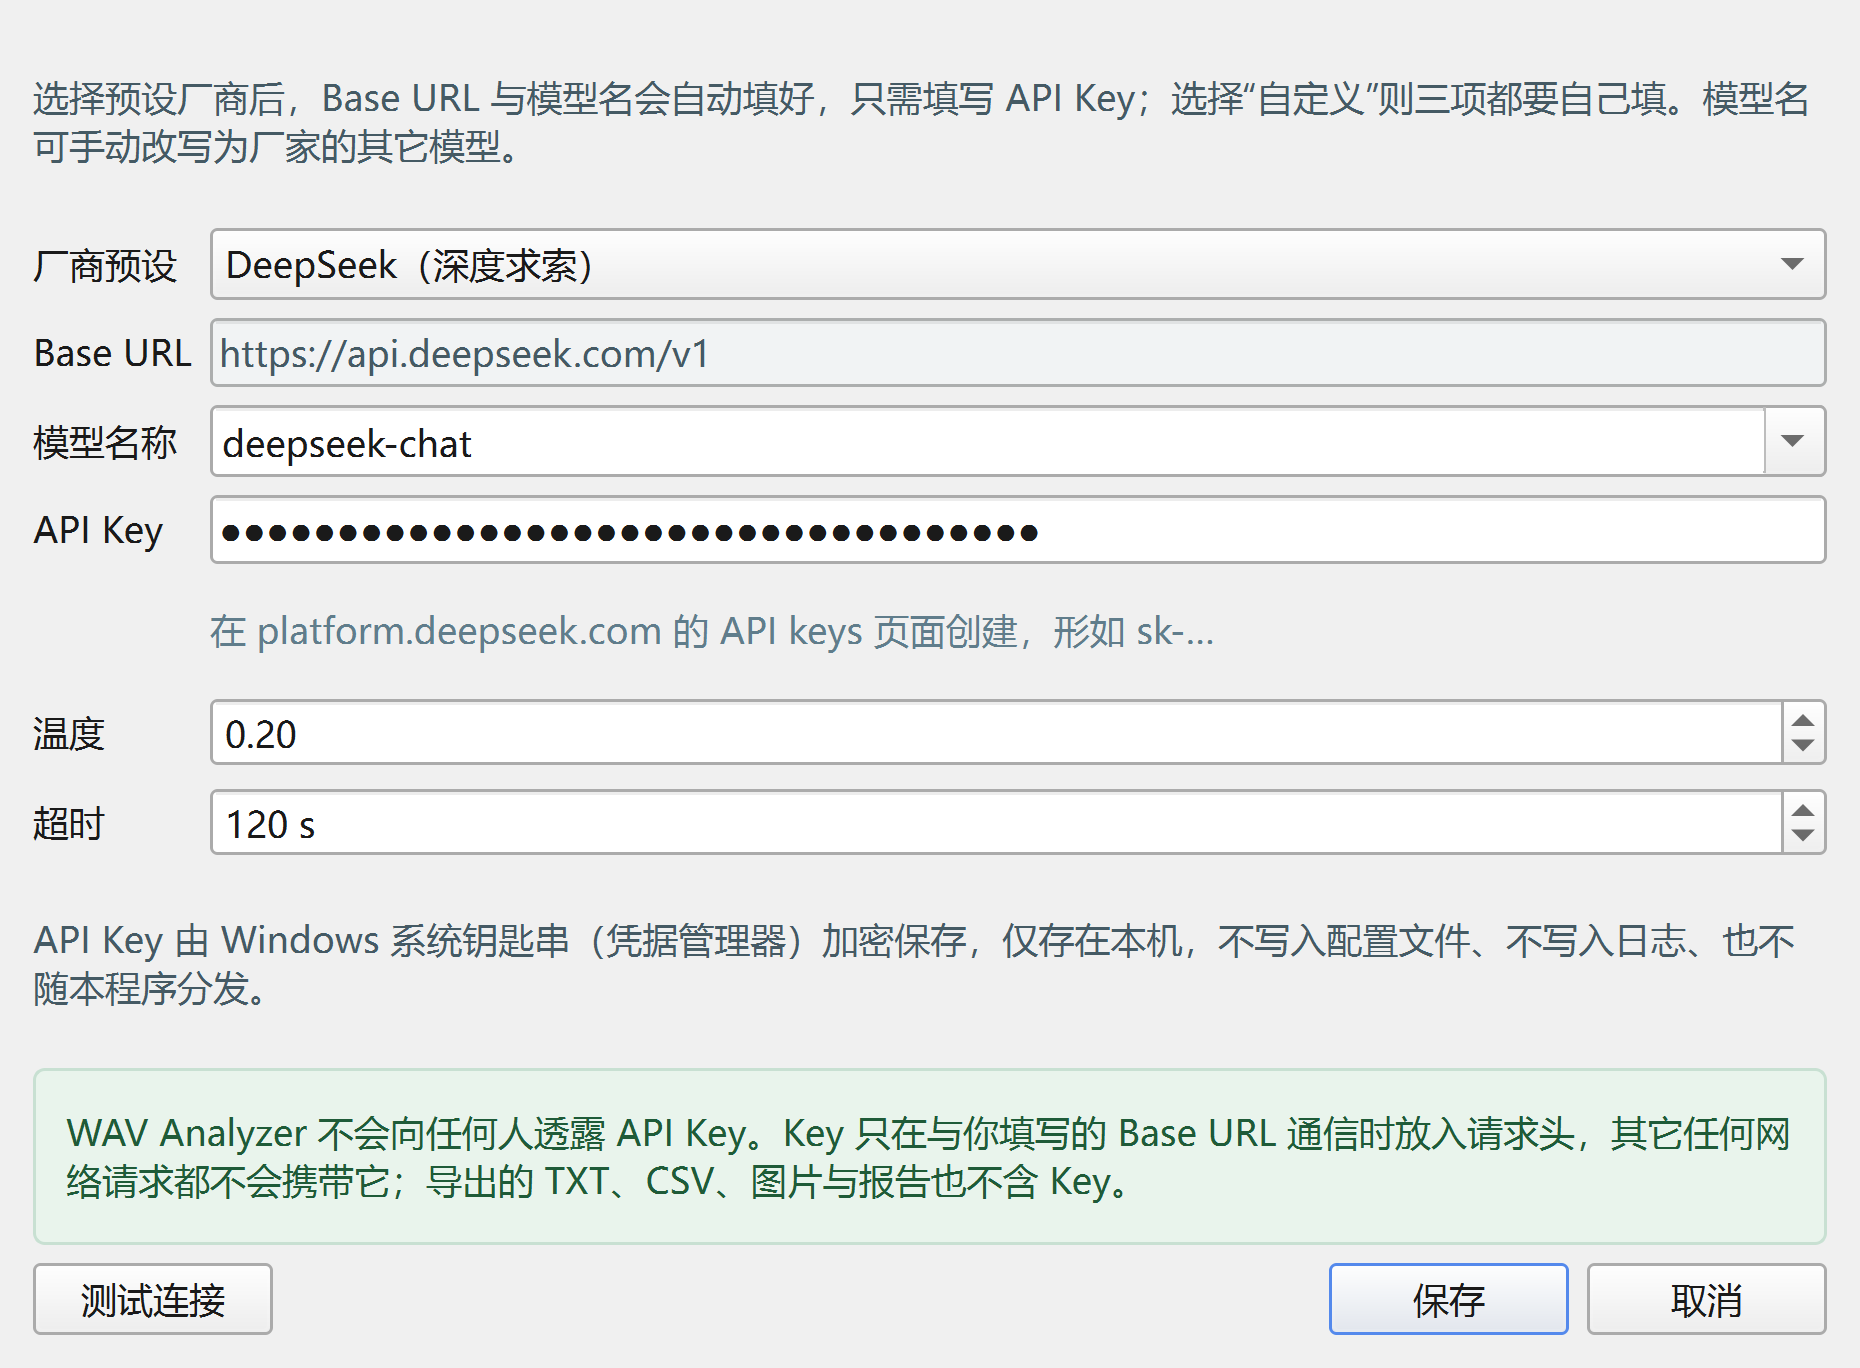
\includegraphics[width=0.88\textwidth]{11_ai_settings.png}
\caption{模型设置对话框。API Key 一栏只显示圆点；下方两段说明分别交代 Key 存在哪里、以及程序会不会把它发给别人。}
\label{fig:ai_settings}
\end{figure}

几点约定：

\begin{itemize}
  \item 选预设厂商时，Base URL 一栏变灰并锁定，避免手改出错；选“自定义”才会解锁。
  \item “模型名称”是可编辑下拉框：既能直接选预设模型，也能改写为厂家发布的其它模型名。
  \item “温度”控制回答的随机性，实验数据处理建议保持默认的 0.2。
  \item “超时”默认 \textbf{120 s}，可在 5--600 s 之间调整。连接阶段另有 15 s 上限：域名解析不了或端口不通时会立刻报错，不用等满两分钟。
\end{itemize}

填写完成后点击“测试连接”，程序会请求 \texttt{/models} 接口验证地址与 Key。

\subsection{API Key 存在哪里}

上一版给过一个“使用 Windows 系统钥匙串保存 Key”的勾选框，实际使用中很别扭：不勾就存不住 Key，每次启动都得重新粘贴一遍。这一版把它去掉，改成固定策略加一句明确声明：

\begin{itemize}
  \item \textbf{API Key 由 Windows 系统钥匙串（凭据管理器）保存}。加密存放于本机，不进配置文件、不进日志，也不随程序或报告分发。
  \item \textbf{WAV Analyzer 不会向任何人透露 API Key}。程序只在与你填写的 Base URL 通信时，把它放进请求头；其它任何网络请求都不携带它。导出的 TXT、CSV、PNG 与 HTML 报告里也没有它。
  \item 保存设置时若钥匙串不可用（极少数受组策略限制的机器），程序会明确提示“Key 未能写入钥匙串”，其余设置照常保存。
  \item 清空 Key 一栏再保存，等价于从钥匙串里删除这条记录。
\end{itemize}

\subsection{会话界面}

右侧面板是一次对话，一次提问一条气泡（图~\ref{fig:ai_chat}）。

\begin{figure}[H]
\centering
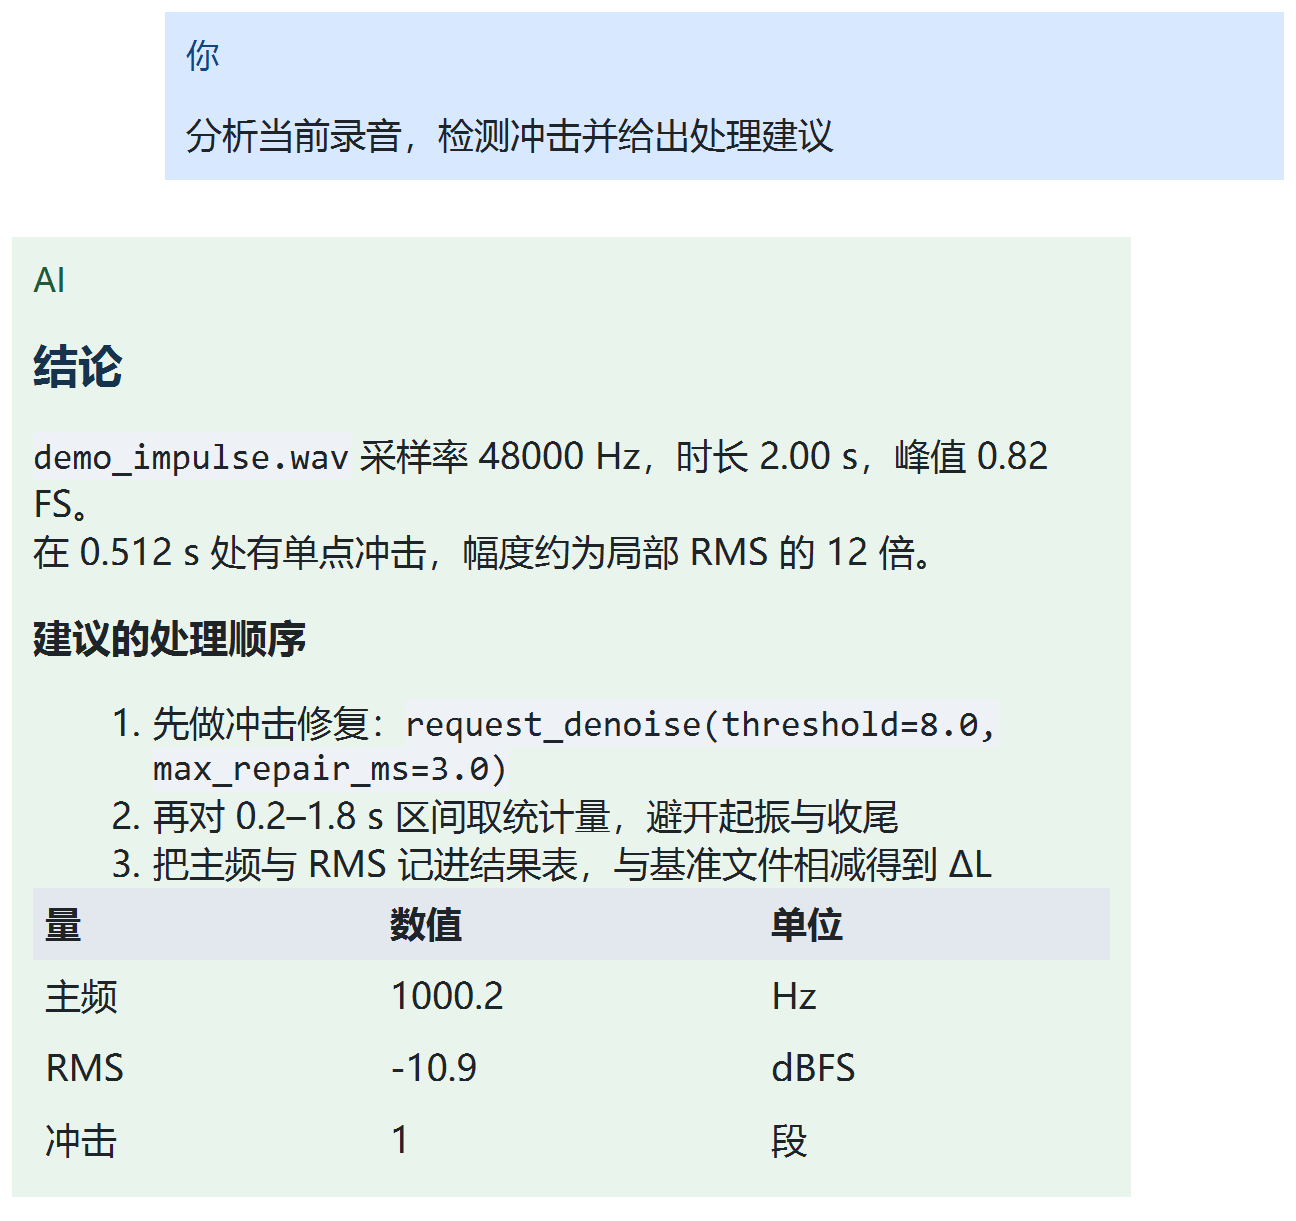
\includegraphics[width=0.64\textwidth]{12_ai_chat.png}
\caption{AI 会话区。提问在右侧蓝色气泡、回答在左侧绿色气泡，提示与错误各有固定颜色。回答里的标题、列表、表格、行内代码与链接都按 Markdown 渲染。}
\label{fig:ai_chat}
\end{figure}

四类气泡用底色区分，扫一眼就知道哪句是自己说的：

\begin{itemize}
  \item \textbf{你}（浅蓝，靠右）：自己的提问，原样显示，不解析 Markdown；
  \item \textbf{AI}（浅绿，靠左）：模型回答，按 Markdown 渲染；
  \item \textbf{提示}（浅黄）：程序给出的中性说明，例如“去噪预览 0 段，已跳过确认”；
  \item \textbf{请求失败}（浅红）：超时、鉴权失败等错误，正文直接写清下一步该怎么做。
\end{itemize}

回答按 Markdown 渲染，因此 \texttt{\#\#}、\texttt{**}、\texttt{|} 这类符号不会原样出现在界面上，而是变成标题、加粗、表格、列表、行内代码与可点击链接。选中文字照常可以复制，跨气泡选择也会连同底色一起带走。

\subsection{受控工具调用}

在输入框中描述任务，例如：“检测当前 WAV 中的冲击，说明处理依据并给出统计结果。”AI 只能调用程序内置的白名单工具，不能执行任意代码。可用工具包括：

\begin{itemize}
  \item 读取当前文件信息与质量报告；
  \item 执行傅立叶分析；
  \item 计算区间统计；
  \item 生成去噪预览。
\end{itemize}

AI 返回的说明只能引用本地工具返回的真实数值，不能编造数据。

\subsection{去噪确认}

AI 请求应用去噪时，程序弹一次确认框，写明事件段数、修复的采样数与排除数，按钮是“应用”与“不应用”，默认停在“不应用”：

\begin{itemize}
  \item \textbf{只问一次}。模型在一轮里可能连续调用多次预览工具，程序取最后一次结果统一确认，不会关掉一个又冒一个。
  \item \textbf{0 段不问}。没检测到需要修复的区段时，弹框毫无意义（点了应用也什么都不变）。这时程序在会话里留一条黄色提示，直接跳过。
  \item \textbf{随时可退出}。点“不应用”、点右上角关闭、按 Esc 都等于放弃，效果一致，不会再次弹窗。
  \item \textbf{只改处理版本}。应用后原始 WAV 不变，且可以撤销。
\end{itemize}

\subsection{隐私与失败处理}

上传给 AI 的默认内容是数值摘要和工具结果，不是完整 WAV 文件。如使用外部模型服务，应遵守相应平台的隐私和数据管理要求，不要把实验原始数据或 API Key 写进聊天内容。

请求失败时程序按原因给不同提示，照提示处理即可：

\begin{itemize}
  \item \textbf{请求超时}：在超时时间内没收到完整响应。推理类模型写长报告时最容易遇到，把“超时”调到 300 s，或改用响应更快的模型。
  \item \textbf{无法连接}：检查网络与代理，并确认 Base URL 是否写全（一般以 \texttt{/v1} 结尾）。
  \item \textbf{401 / 402 / 403 / 404 / 429}：分别对应 Key 无效、余额不足、无该模型权限、地址或模型名不存在、限流或额度用尽。
\end{itemize}

AI 不可用时，程序的手动分析、去噪、统计、批量处理与导出功能完全不受影响。

% ==================== 第 15 章 ====================
\section{结果导出与报告}

\subsection{五项导出功能}

左侧“导出”分组提供五项输出：

\begin{table}[htbp]
\centering
\caption{导出功能说明}
\begin{tabular}{@{}l p{8.4cm}@{}}
\toprule
功能 & 输出内容 \\
\midrule
导出处理后 WAV & 当前内存中的处理版本，不覆盖原始文件 \\
导出分析 TXT & 定宽对齐的纯文本分析报告，可直接导入 Origin、Excel、Python \\
导出图像 PNG & 波形图、频谱图或时频图，论文版式或屏幕版式 \\
导出当前统计 CSV & 当前选区的统计结果 \\
生成独立 HTML 报告 & 波形、频谱、统计、包络、去噪记录和 AI 说明 \\
\bottomrule
\end{tabular}
\end{table}

\subsection{导出分析 TXT}

点击“导出分析 TXT…”，弹出如图~\ref{fig:txt-dialog} 的设置窗口。

\begin{figure}[H]
\centering
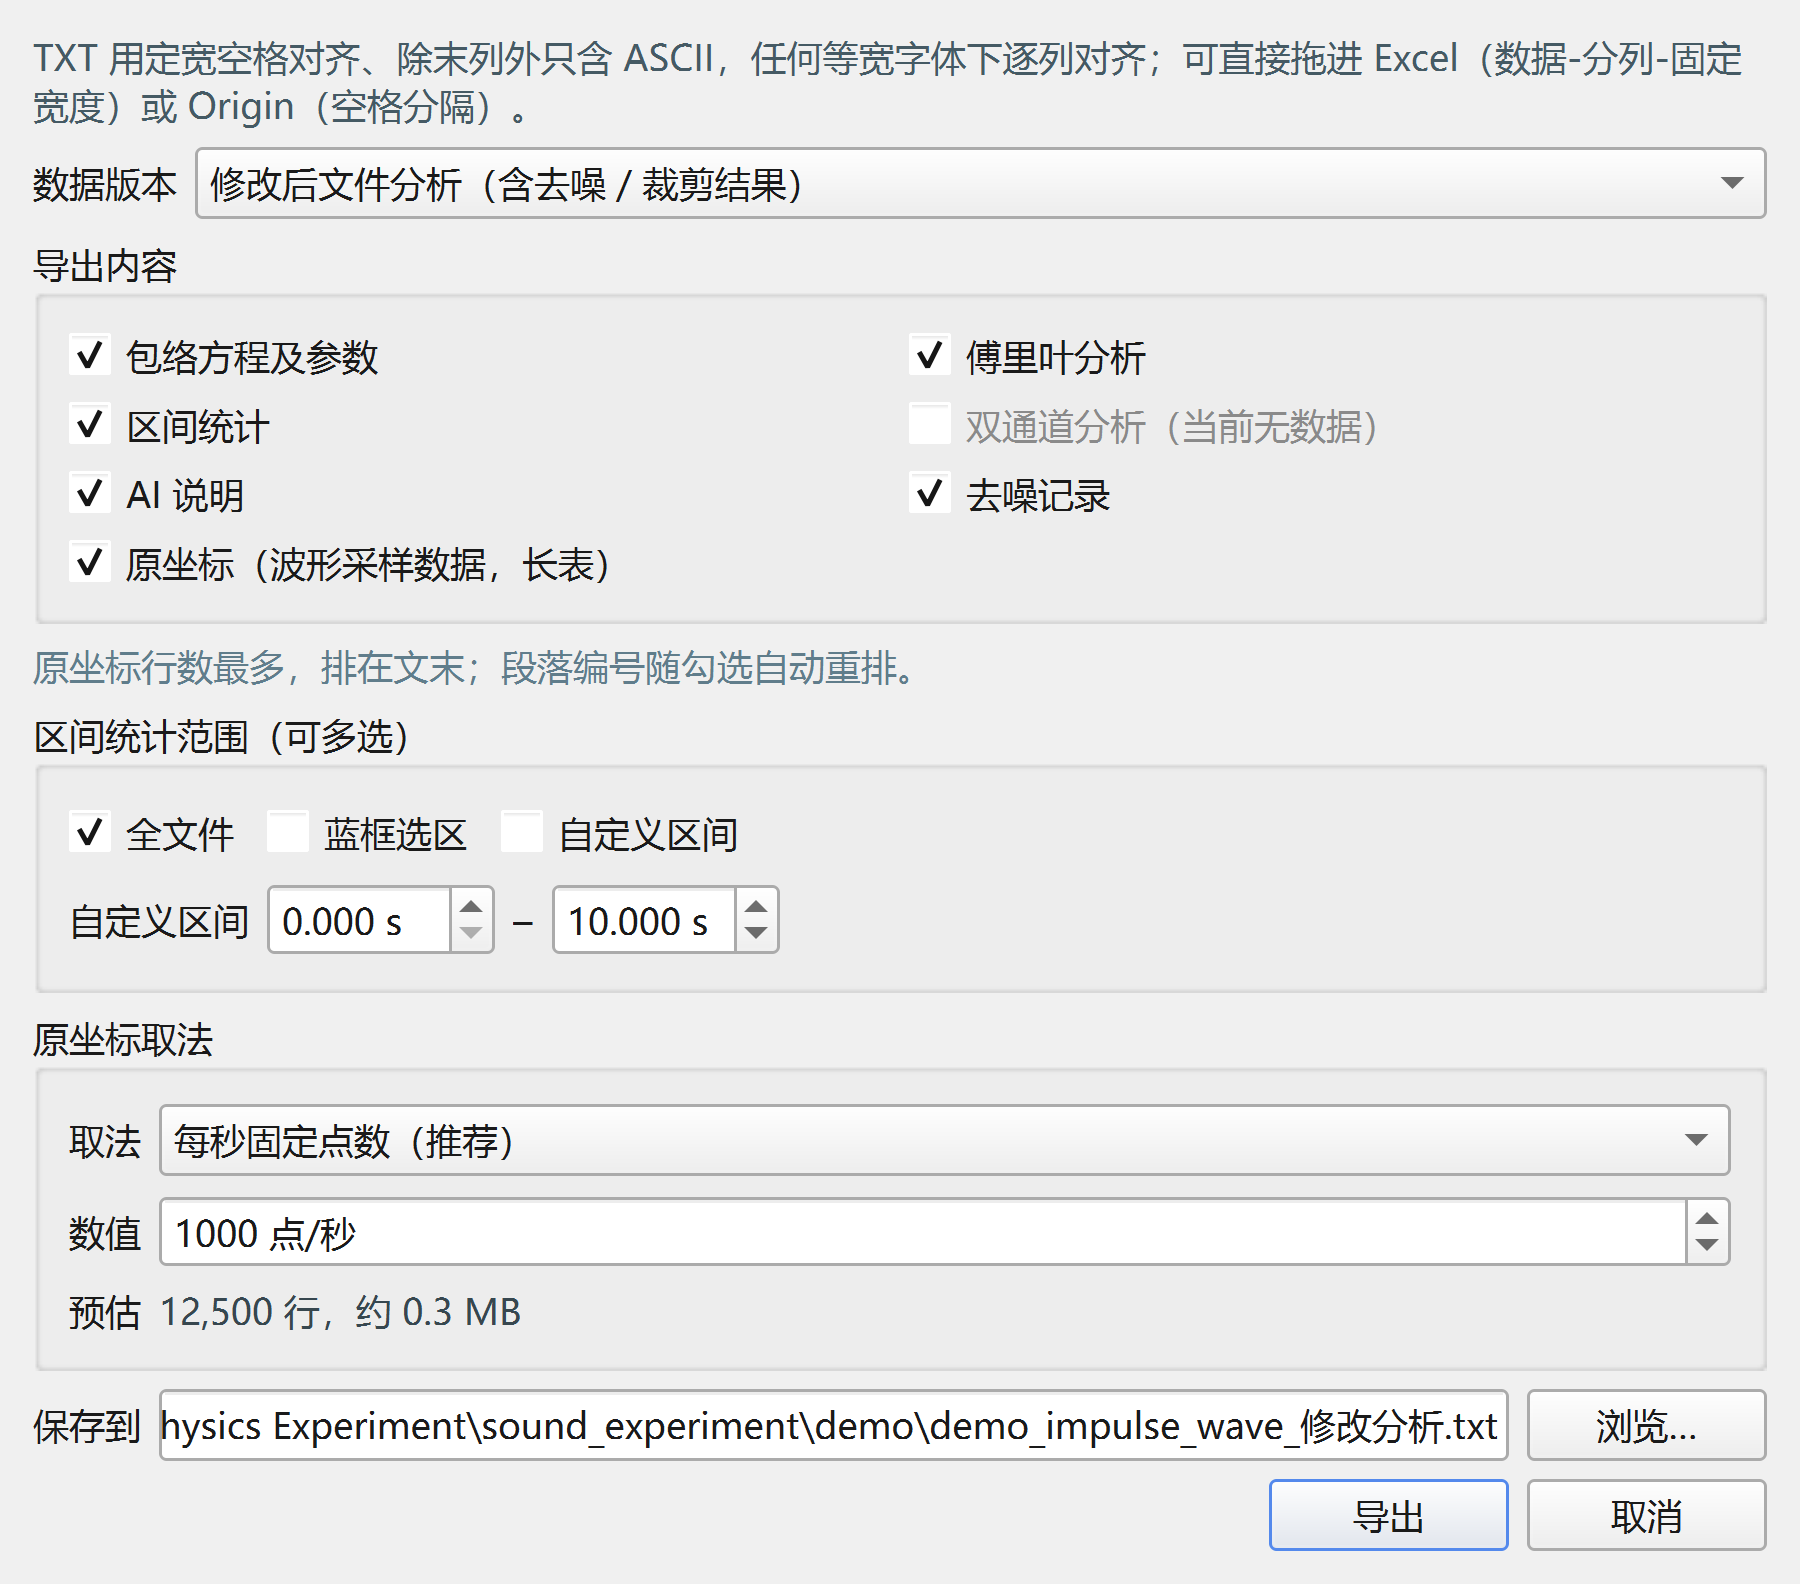
\includegraphics[width=0.78\textwidth]{08_txt_export_dialog.png}
\caption{导出分析 TXT 对话框：数据版本、章节勾选、区间统计范围与坐标取法}
\label{fig:txt-dialog}
\end{figure}

窗口上要定三件事：用哪个数据版本、导出哪些章节、坐标怎么取。默认文件名跟随数据版本：

\begin{itemize}
  \item 选“源文件分析（未做任何编辑）”时，输出 \texttt{原始文件名\_源文件分析.txt}，数据取磁盘上的原始 WAV，不掺入当前窗口里改过的内容。
  \item 选“修改后文件分析（含去噪／裁剪结果）”时，输出 \texttt{原始文件名\_修改分析.txt}，数据取当前内存中的处理版本，并附去噪记录。
\end{itemize}

\subsubsection*{七个章节，序号随勾选自动重排}

文件内容按固定顺序排列，越长的表越靠后，方便打开文件就能读到关键结论：

\begin{table}[htbp]
\centering
\caption{分析 TXT 的章节顺序}
\begin{tabular}{@{}clp{7.2cm}@{}}
\toprule
序 & 章节 & 内容 \\
\midrule
1 & 包络方程及参数 & 选区、提取方法、拟合模型、拟合方程、$R^2$、RMSE、参数表、约 24 行包络抽样 \\
2 & 傅里叶分析 & 窗函数、FFT 点数、频率分辨率、主频、THD；主要谱峰表、谐波表、完整谱表抽样 \\
3 & 区间统计 & 每段选定区间的全部统计量，附中文名与释义 \\
4 & 双通道分析 & 互相关时延、峰值质量、两路电平、AGC 风险提示 \\
5 & AI 说明 & AI 助手生成的处理说明正文 \\
6 & 去噪记录 & 阈值、检测段数、插值／排除段数、逐段起止时间与峰值偏差（长表） \\
7 & 原坐标 & 逐采样点或抽稀后的 $t$、$x$、$L$ 三列（长表，通常占总行数九成以上） \\
\bottomrule
\end{tabular}
\end{table}

没勾的章节不输出，剩余章节的编号会自动连续重排，不会留下空号。当前没有数据的章节会在复选框上标注“当前无数据”并禁用，避免勾了却导出一段“未计算”。

\subsubsection*{为什么不用制表符}

程序内部统一用\textbf{定宽空格}对齐，全文没有一个制表符，原因是两条实测结论：

\begin{enumerate}
  \item 制表符只能跳到 8 的整数倍位置。字段一长就会跨过制表位，其后整列错位，而坐标表的数值长度是随数据变化的。
  \item “一个汉字等于两个等宽字符”并不成立。实测 Consolas 加中文回退为 1.875 格，SimSun 为 1.818 格。按 2 格补空格，每多一个汉字就少补 0.125 格，中文列之后整列持续左漂。
\end{enumerate}

因此规定：\textbf{除末列外只允许 ASCII 字符}。ASCII 在任何等宽字体下都恒定占 1 格，列起点与字体、字号、编辑器无关。中文只出现在最后一列，或者以 \texttt{\#} 开头的注释行里；表头用 \texttt{t/s}、\texttt{x/FS}、\texttt{L/dBFS}、\texttt{idx}、\texttt{key}、\texttt{value} 这类缩写，中文全名写在表格上方的 \texttt{\# 列定义：…} 行。程序的排版函数对非末列的中文会直接报错，防止后续改动把对齐破坏掉而无人察觉。

%% minipage 包住，避免代码块被分页切成两半（列对齐示例被切开就没法看了）。
\begin{center}
\begin{minipage}{0.96\textwidth}
\begin{lstlisting}
# 列定义：t/s 时间（秒）  x/FS 幅值（满幅归一化）  L/dBFS 电平 20lg|x|
t/s             x/FS   L/dBFS
0.000000   +0.001526   -56.3291
0.000023   +0.004578   -46.7843
0.000045   +0.007629   -42.3496
\end{lstlisting}
\end{minipage}
\end{center}

\subsubsection*{坐标表取法}

“原坐标”是全文件最长的部分，导出前必须选一种取法：

\begin{table}[htbp]
\centering
\caption{坐标表三种取法}
\begin{tabular}{@{}l p{4.1cm} p{5.4cm}@{}}
\toprule
取法 & 换算方式 & 适用场景 \\
\midrule
每秒固定点数（默认 1000） & 步长 $=$ 采样率 $/$ 每秒点数 & 常规分析，各文件行数可比 \\
按步长抽稀 & 步长 $=$ 指定采样点数 & 需要精确控制抽样间隔 \\
全部采样点 & 步长 $=$ 1 & 需要重采样、重做频谱或逐点核对 \\
\bottomrule
\end{tabular}
\end{table}

对话框会实时估算行数与文件体积。选择“全部采样点”且预计超过 500 万行时，程序会再弹一次确认，因为 48\,kHz 双声道一小时的录音全量导出会达到上亿行、数 GB 级别。生成过程按每批 8192 行写盘，不在内存里拼出整份字符串：4000 万点全量导出若一次性拼接约需 3.5\,GB 内存，分批后峰值占用只有几十 MB。

\subsubsection*{区间统计可多选}

“区间统计范围”支持同时勾选多项：全文件、蓝框选区、自定义区间（起止时间可手填）。勾了几项就输出几段统计，每段独立成块并标注区间。当前没有蓝色选区时，“蓝框选区”一项会改名为“蓝框选区（当前无选区）”并禁用。

\subsubsection*{文件格式约定}

\begin{itemize}
  \item 编码 UTF-8 带 BOM，Windows 记事本与 Excel 双击打开都不乱码。
  \item 以 \texttt{\#} 开头的行为说明文字，不含数据，导入时可整体忽略。
  \item 单位缩写：FS 为数字满幅归一化幅值，dBFS 为 $20\lg(|x|/\mathrm{FS})$；dBFS 不等于声压级 dB SPL。
  \item \texttt{-inf} 表示该点幅值为 0、对数无定义；\texttt{nan} 表示该量在本数据上不可计算。
  \item 文件头记录源文件完整路径、采样率、声道数、总采样点、编辑次数与源 WAV 的 MD5 指纹（为免读整份长文件，取前 256\,MB 计算、输出前 16 位），用于核对这份导出与原始录音是否对应。
  \item 文末“导出说明”段汇总编码、对齐规则、导入方法与本次坐标步长。
\end{itemize}

导入示例：Python 用 \texttt{pandas.read\_csv(path, sep=r"\textbackslash s+", comment="\#")}；Excel 用“数据 → 分列 → 固定宽度”；Origin 导入时选空格分隔并忽略 \texttt{\#} 行。

\subsection{导出图像 PNG}

点击“导出图像 PNG…”，弹出如图~\ref{fig:export-dialog} 的设置窗口。图像类型默认跟随当前标签页（波形与选区页给出波形图，傅立叶分析页给出频谱图，时频图页给出时频图），随后勾选要画的内容：

\begin{figure}[H]
\centering
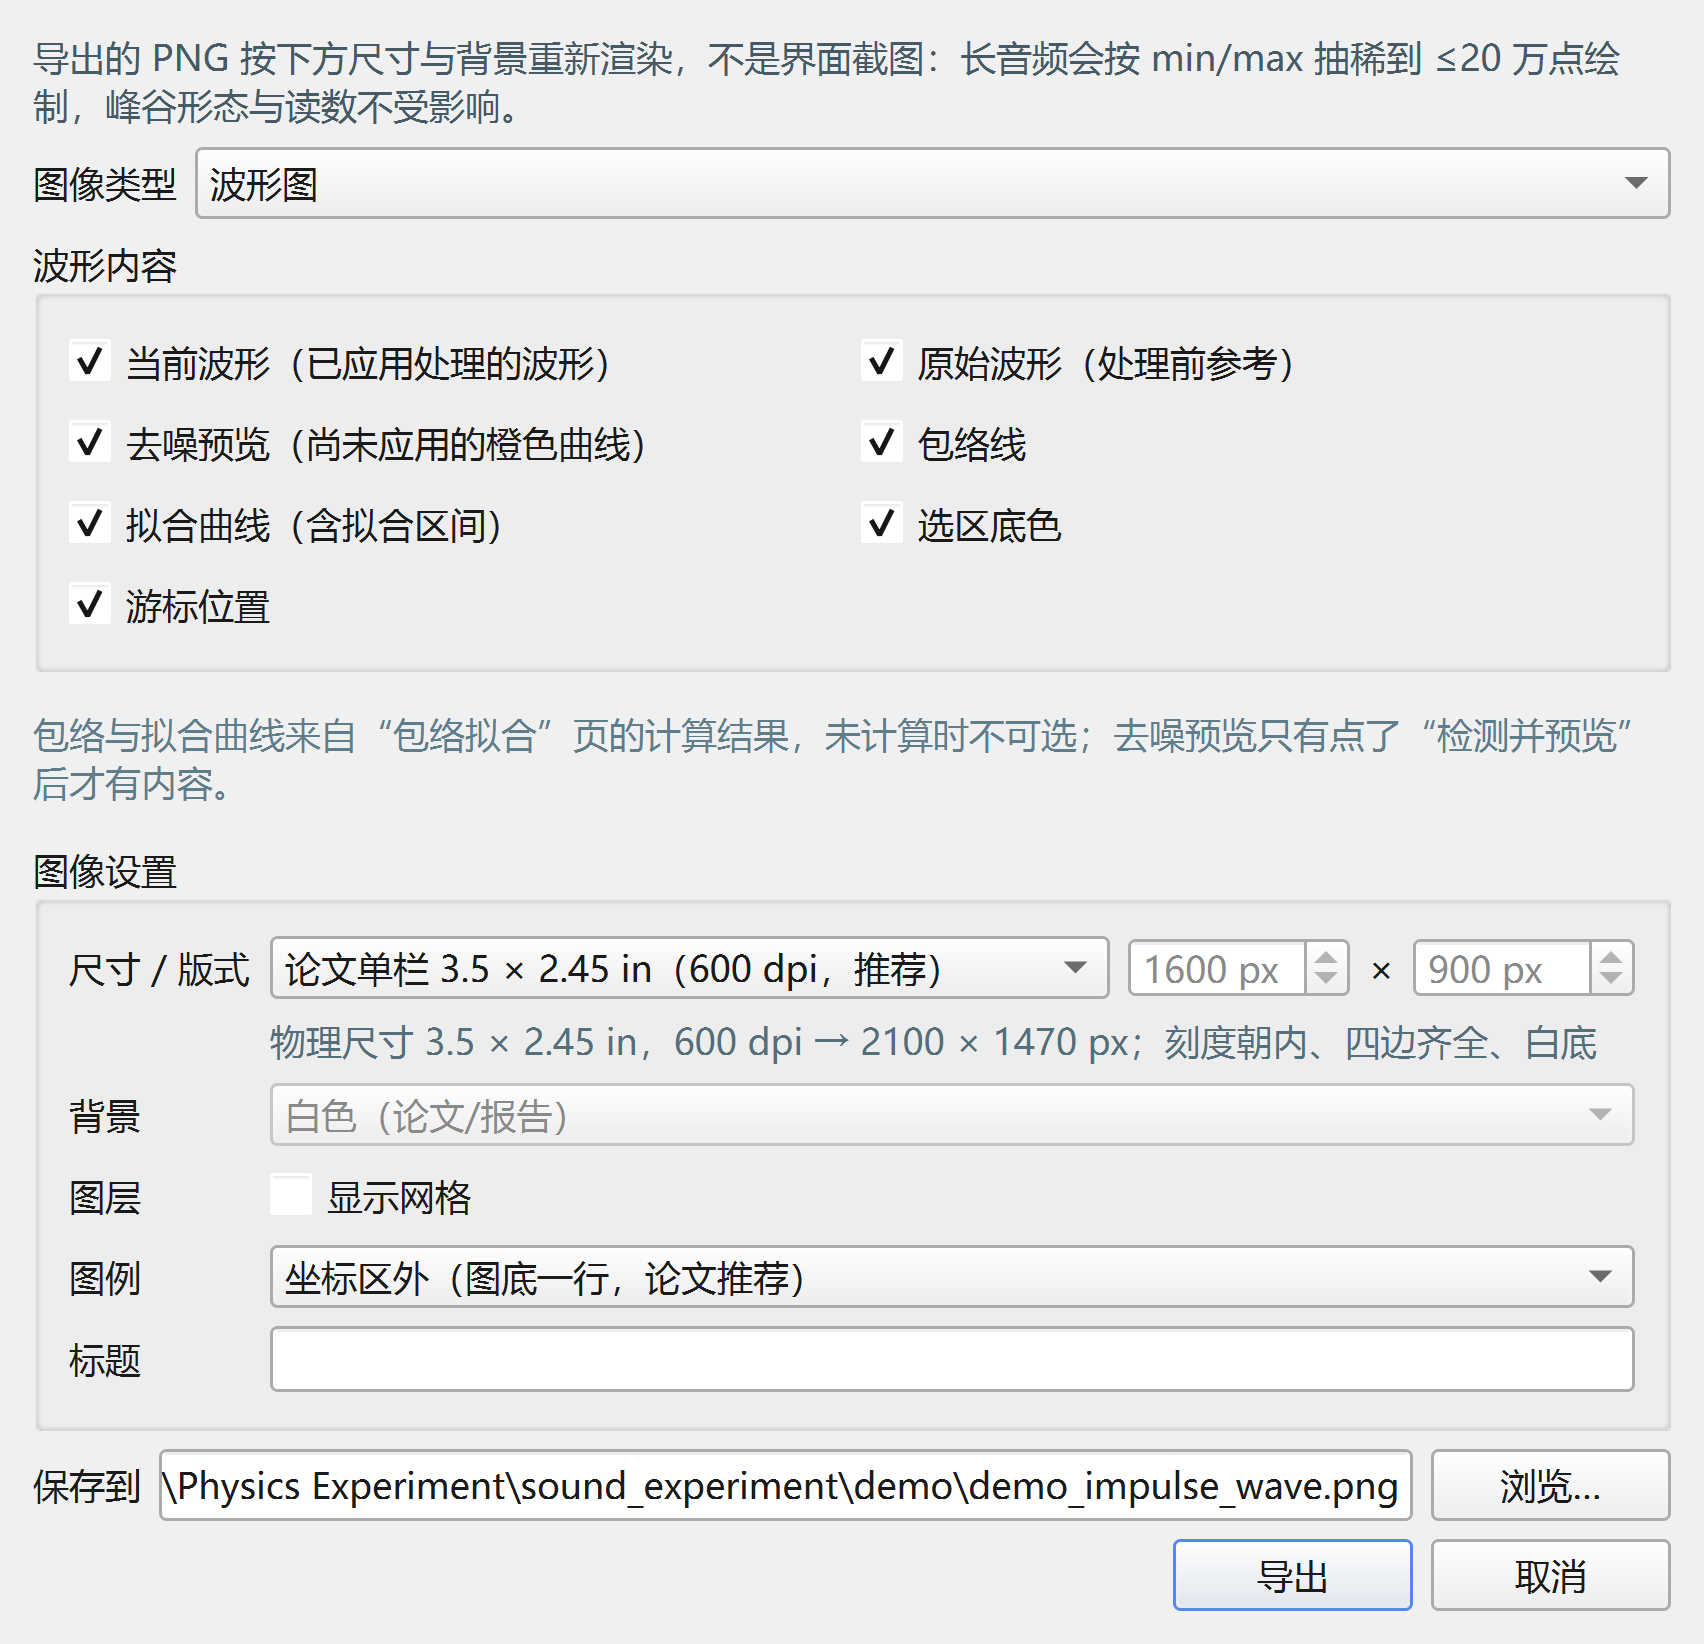
\includegraphics[width=0.66\textwidth]{07_export_dialog.png}
\caption{导出图像对话框：图像类型、内容勾选与输出设置}
\label{fig:export-dialog}
\end{figure}

\begin{itemize}
  \item \textbf{波形图}：当前波形（必选）、原始波形、去噪预览、包络线、拟合曲线、选区底色、游标位置。当前没有数据的项会标注“当前无数据”并禁用，避免勾了却画不出来。
  \item \textbf{频谱图}：纵轴可选 dBFS 或线性幅值，可限制频率上限、标注主要谱峰、标出基频整数倍位置，并可附带相位谱子图。
  \item \textbf{时频图}：可限制频率上限，并调整色标下限（默认 $-100$\,dBFS），调低可看清更弱的成分。
\end{itemize}

\subsubsection*{两种版式}

尺寸下拉框分为论文版式与屏幕版式两组，二者输出参数完全不同：

\begin{table}[htbp]
\centering
\caption{论文版式与屏幕版式的区别}
\begin{tabular}{@{}lll@{}}
\toprule
项目 & 论文版式 & 屏幕版式 \\
\midrule
尺寸依据 & 物理尺寸（英寸） & 像素 \\
单栏 & $3.50 \times 2.45$\,in & -- \\
双栏 & $7.00 \times 2.60$\,in & 1600$\times$900 / 1920$\times$1080 \\
分辨率 & 固定 600\,dpi & 由像素尺寸决定 \\
字号 & 正文 8.5\,pt，标注 7.5\,pt & 跟随屏幕 \\
背景 & 强制白色 & 白／深色／透明可选 \\
\bottomrule
\end{tabular}
\end{table}

论文版式按期刊双栏排版的通行尺寸给出，插入 \LaTeX{} 或 Word 双栏正文时不需要再缩放，字号线宽也不会因为缩放而失真。单栏版式下如果同时勾了包络或拟合曲线，程序会自动拆成上下两个子图（上波形、下包络），高度按 1.32 倍比例放大，两条曲线各自有充足的纵向空间；屏幕版式仍然画在同一张图里。

屏幕版式下可选背景“白色／深色／透明”。选深色适合投影；选透明时输出带 alpha 通道的 PNG，可直接叠放到其它版面。论文版式强制白底，因为期刊排版几乎不接受深色或透明底图，留这个选项只会造成误用。

\subsubsection*{图例与制图规范}

图例默认放在\textbf{坐标区外、图底一行}，横向排列，不遮挡任何曲线。这一点对双图版式尤其重要：上下两个子图共用一行图例，三种曲线名（波形、包络、拟合）都在，不会被上面的子图截掉一半。也可以在“图例位置”里改为“坐标区内右上角”或“不显示图例”。

\begin{itemize}
  \item 与界面共用同一份数据与同一套 min/max 抽稀规则。长音频在绘制前抽稀到不超过 20 万点，只影响线条密度，峰谷形态与坐标读数不受影响，单条曲线也不会有视觉缺失。
  \item 字体遵循学术制图规范：中文宋体，西文与数字 Times New Roman；变量斜体（$t$、$x$、$A$、$L$、$f$、$\varphi$），单位正体（s、Hz、FS、dBFS、rad）。
  \item 论文版式的刻度朝内，四条边框刻度齐全并带次刻度，这是期刊插图与学位论文插图的常见要求。
  \item 包络曲线在绘图时做 5\,ms 滑动平均平滑，只改善观感；拟合所用的数据和统计结果仍是未平滑的原始包络，平滑不改变任何数值结论。
  \item 幅值谱里的谐波位置用峰顶小三角加 $f_0$、$2f_0$…… 标注，白底文字框避免压住谱线；离边框太近的峰会自动左移或抬高，不会被裁掉。已被谐波标注覆盖的位置不会再重复标一次谱峰频率。
  \item 时频图在论文版式下使用 magma 色表并做光栅化处理，色标刻度朝内，嵌入 PDF 后文件体积更小。
  \item 导出过程在工作线程中完成，期间显示“处理中”遮罩，长音频约需 1--3 秒。
\end{itemize}


\subsection{HTML 报告内容}

独立 HTML 报告由程序自动生成，内容包括：文件基本信息、处理步骤与参数、傅立叶分析结果、区间统计量、包络方程与拟合优度、冲击检测与修复记录、AI 生成的处理说明。报告明确标注 dBFS 与 dB SPL 的区别，避免单位误用。

该报告由本程序独立生成，不参考工作区内其他实验报告的格式和内容。可以直接在浏览器中打开，也可以通过“打印 → 另存为 PDF”转换为 PDF 格式。

% ==================== 第 16 章 ====================
\section{批量处理}

\subsection{为什么需要批量}

隔音箱开孔实验动辄上百个录音：五块孔径板乘四个频率乘三次重复已经是六十个，加上密封基准、形状组和距离组，一百四十多个文件是常态。用单文件界面逐个处理，改频率、框选区、抄读数全靠手点，一个文件两分钟，整批就是五六个小时，而且抄错一位数很难被发现。

批量处理把“做哪些步骤、每步用什么参数”抽成一条可保存的流水线：配一次，整批执行，直接输出一张一行一个文件的统计表。全程只读源文件，处理期间界面不会假死。

\subsection{设计约束}

\begin{itemize}
  \item \textbf{选择文件只记路径，不导入}。点“选择待处理的文件”后程序只保存路径字符串，几百个文件也是瞬时响应；真正的读取发生在点“开始处理”之后。
  \item \textbf{引擎与界面分离}。批量引擎不引用任何界面模块，跑在独立工作线程里；主窗口只显示进度，因此处理大文件时界面不会假死。
  \item \textbf{每个文件独立状态}。裁剪、去噪、包络都作用在该文件自己的数据副本上，绝不共用数组；前一个文件的处理结果不可能污染下一个。
  \item \textbf{源文件始终只读}。批量只写“导出”类步骤指定的新文件，不碰源 WAV。
  \item \textbf{单个文件失败不中断整批}。某个文件读不出来或参数不适用时，只把该文件标记为失败并记入汇总，其余照常处理。
\end{itemize}

\subsection{界面与操作顺序}

在主界面左侧“批量处理”分组里点“批量处理…”，打开脚本编辑窗口（图~\ref{fig:batch_dialog}）。

\begin{figure}[H]
\centering
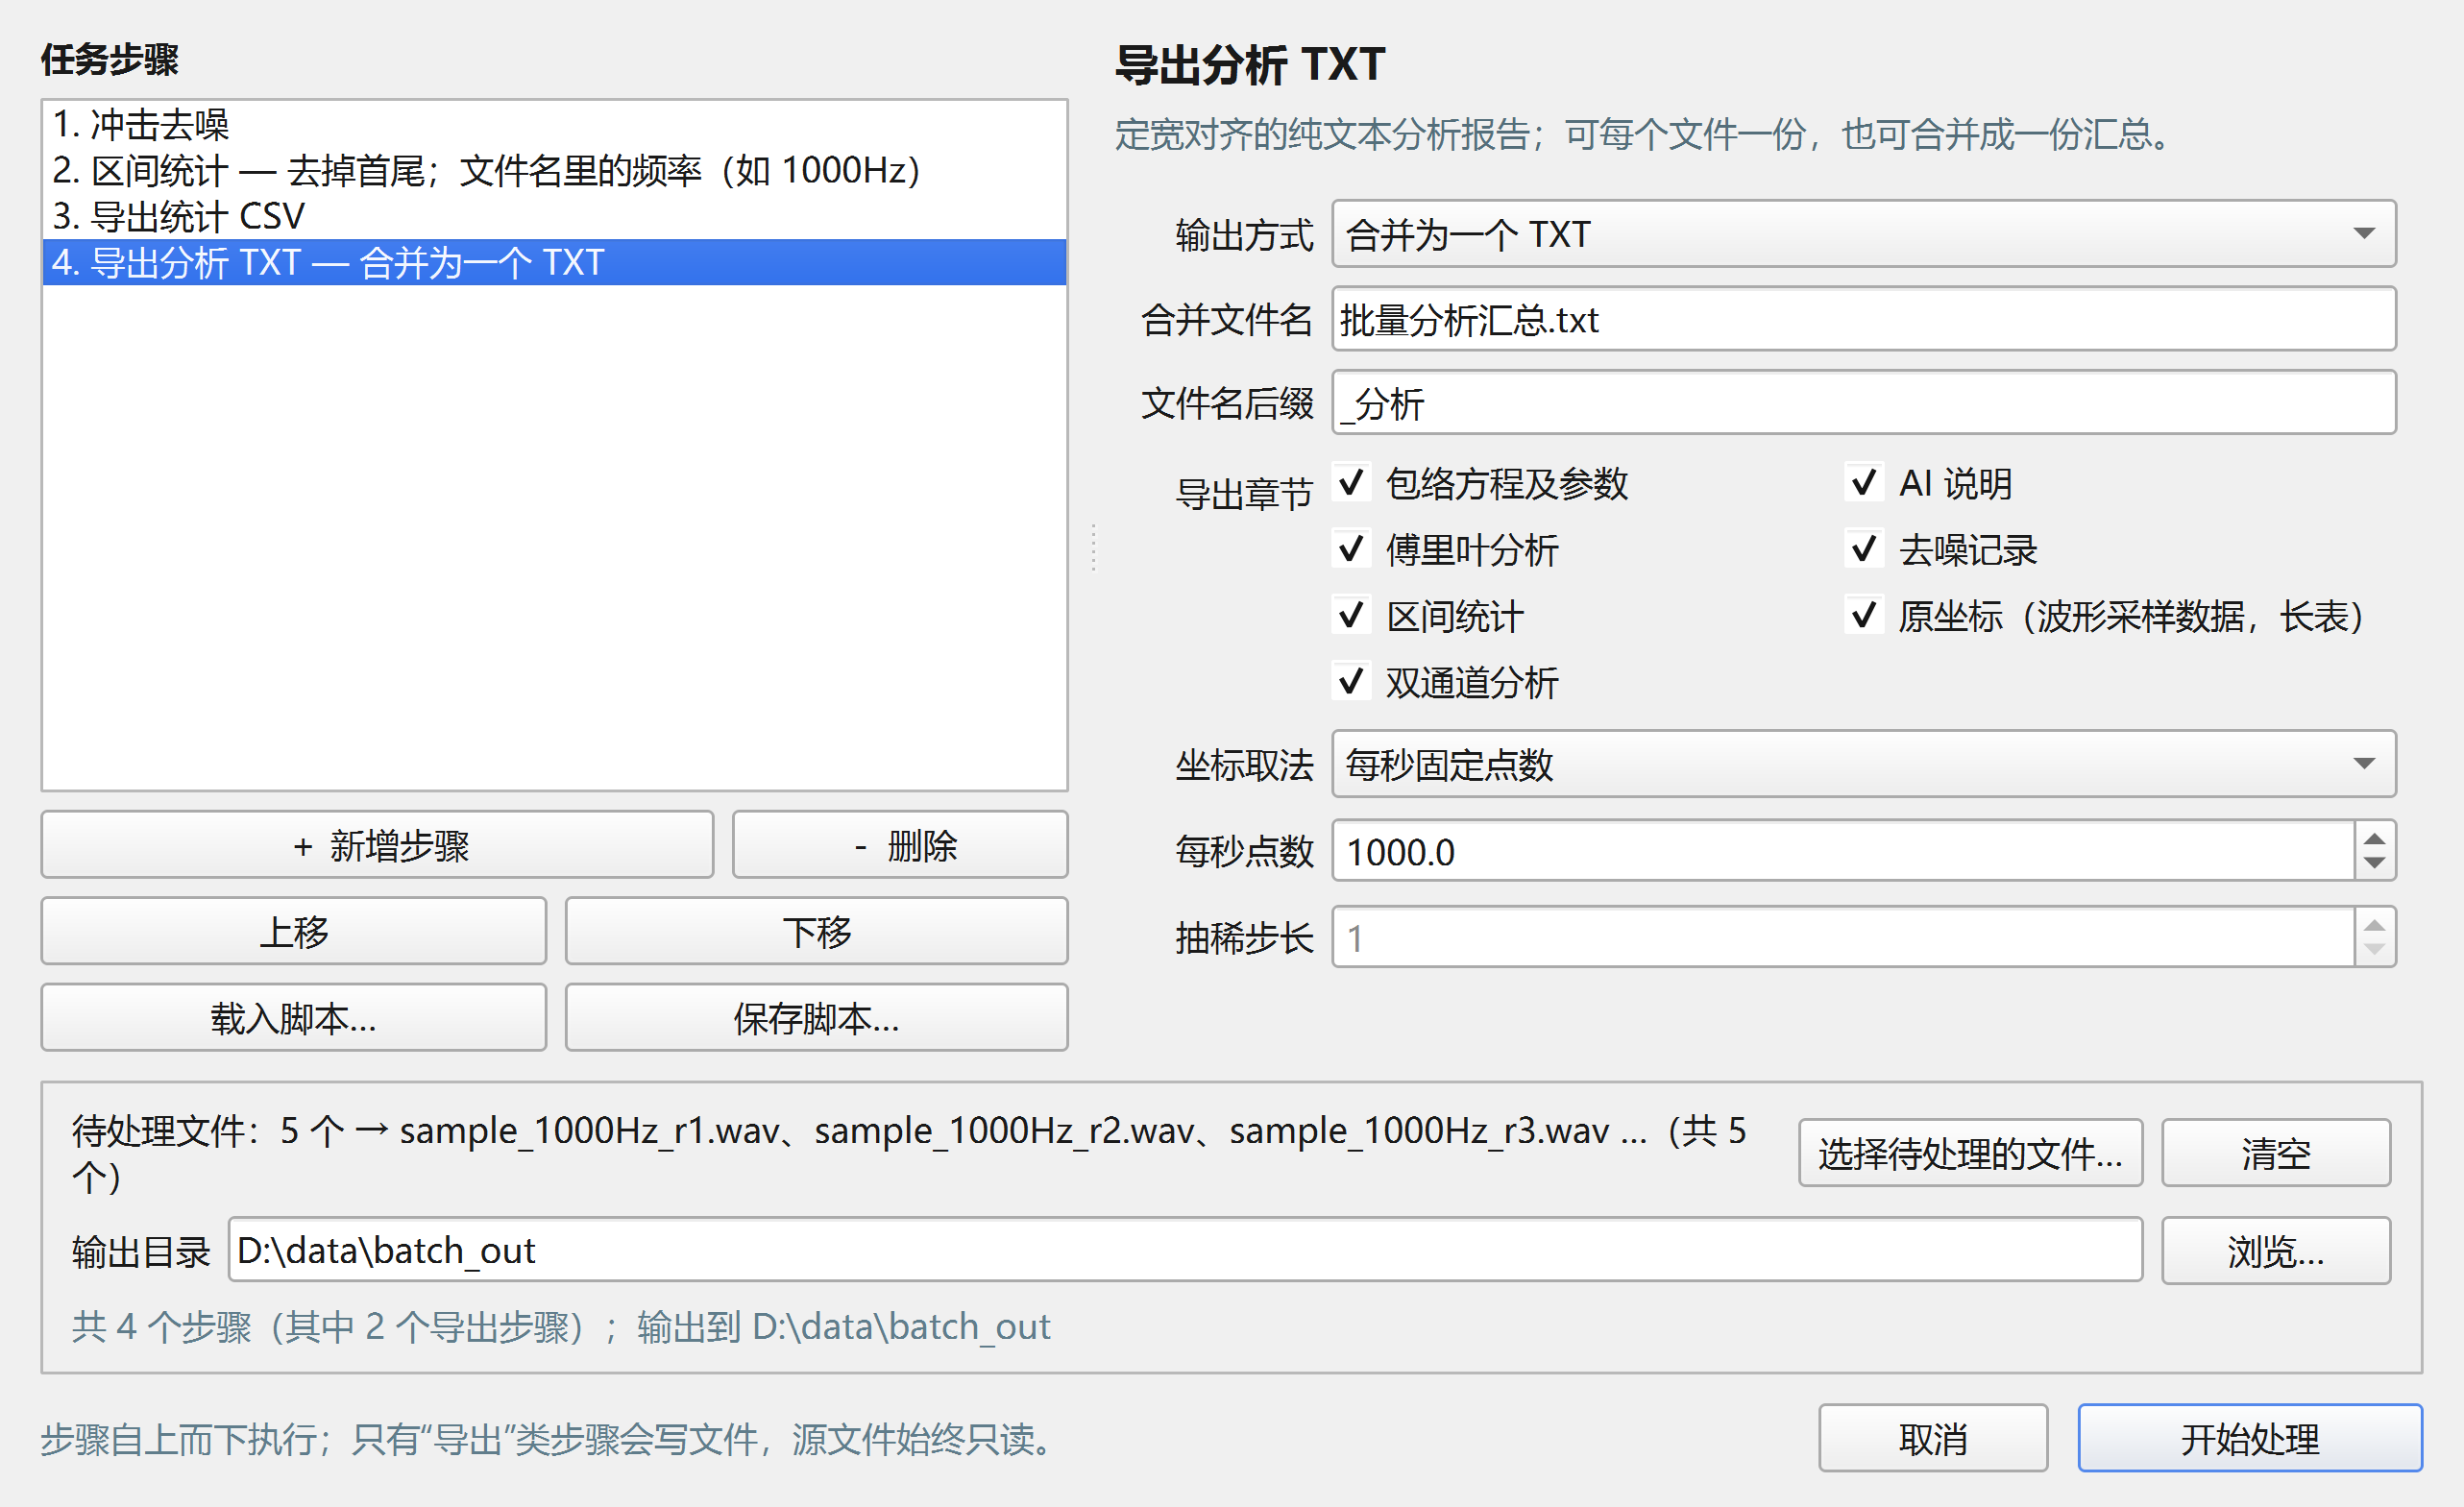
\includegraphics[width=0.86\textwidth]{09_batch_dialog.png}
\caption{脚本编辑窗口。左栏步骤自上而下执行，右栏是当前选中步骤的参数，下栏是待处理文件与输出目录。}
\label{fig:batch_dialog}
\end{figure}

操作顺序固定为六步：

\begin{enumerate}
  \item 点“＋ 新增步骤”，从菜单里挑一个功能，右栏立刻出现该步骤的参数；
  \item 设好参数；当前组合下无意义的参数会自动置灰（选“每个文件一个 TXT”时“合并文件名”不可用，选“每秒固定点数”时“抽稀步长”不可用）；
  \item 需要调整顺序时用“上移”“下移”，不需要的步骤用“－ 删除”；
  \item 点“选择待处理的文件”多选 WAV，只记录路径；
  \item 填输出目录；留空表示写到源文件同目录，一般建议单独指定一个空目录；
  \item 点“开始处理”。
\end{enumerate}

左栏每一行是“序号 + 步骤名 + 非默认参数摘要”，摘要里没有出现的参数就是默认值，不必逐项核对。

\subsection{步骤一览}

十种步骤覆盖单文件界面的全部功能，见表~\ref{tab:batch_steps}。

\begin{table}[htbp]
\centering
\caption{批量处理支持的步骤}
{\small
\begin{tabular}{@{}>{\raggedright\arraybackslash}p{4.0cm}>{\raggedright\arraybackslash}p{4.6cm}>{\raggedright\arraybackslash}p{5.4cm}@{}}
\toprule
步骤 & 主要参数 & 说明 \\
\midrule
冲击去噪 & 阈值、修复长度、范围 & 与单文件去噪同一算法 \\
裁剪到区间 & 起点、终点 & 真正切数据，后续步骤基于裁剪后结果 \\
包络拟合 & 模型、统计区间 & 与单文件包络同一算法 \\
区间统计 & 区间、已知激励频率 & 主频与 THD 受频率约束 \\
双通道时延与电平 & 已知激励频率 & 单声道文件自动跳过 \\
导出处理后 WAV & 后缀、采样格式 & 源文件不动，另存新文件 \\
导出分析 TXT & 输出方式、章节、坐标取法 & 支持合并为一个文件 \\
导出图像 PNG & 图像类型、版式 & 论文单栏／双栏／屏幕 \\
导出统计 CSV & 输出方式 & 默认合并为一张表 \\
生成 HTML 报告 & 文件名后缀 & 每个文件一份独立报告 \\
\bottomrule
\end{tabular}}
\label{tab:batch_steps}
\end{table}

有两个参数在批量里的用法与单文件界面不同，需要特别注意：

\begin{itemize}
  \item \textbf{统计区间}三选一：“全文件”“去掉首尾”“固定区间”。“去掉首尾”对定长录音最省事，起振瞬态与收尾截断一次跳过；它只改变统计范围，不动数据本身，与“裁剪到区间”不是一回事。
  \item \textbf{已知激励频率}三选一：“自动估计（取最强峰）”“固定值（所有文件相同）”“文件名里的频率”。最后一项从文件名里识别 \texttt{1000Hz}、\texttt{2kHz} 这类片段，适合按频率命名的一批录音——一个脚本就能同时处理 500\,Hz 与 4000\,Hz 的文件，不必按频率分批跑。
\end{itemize}

\subsection{合并导出}

TXT 与 CSV 两种导出都提供“合并为一个文件”选项，这是批量处理最常用的输出形式。

\begin{itemize}
  \item \textbf{CSV 默认合并}：一行一个文件，列是二十一项统计量。不同频率、不同板的文件放在一起，直接进 Excel 做透视，或进 Origin 画曲线。
  \item \textbf{TXT 合并}：每个文件的完整报告按处理顺序依次追加进同一个文件，开头是一份文件清单，每段以“分析数据导出”标题开始，带各自的源文件名、路径与 MD5 指纹。合并时\textbf{必须取消“原坐标”段}——每文件五千行坐标，一百多个文件就是几百兆，既打不开也没人看。
\end{itemize}

追加时使用不带 BOM 的 UTF-8。若沿用带 BOM 的写法，每追加一次就会在文件中间插一个零宽字符，在记事本里表现为每段标题前多出一个小方块。

\subsection{运行与进度}

点“开始处理”后，主窗口先被抓成一张快照并做模糊处理当背景，上面浮出一张进度卡片（图~\ref{fig:batch_progress}），批处理期间界面不可操作。

\begin{figure}[H]
\centering
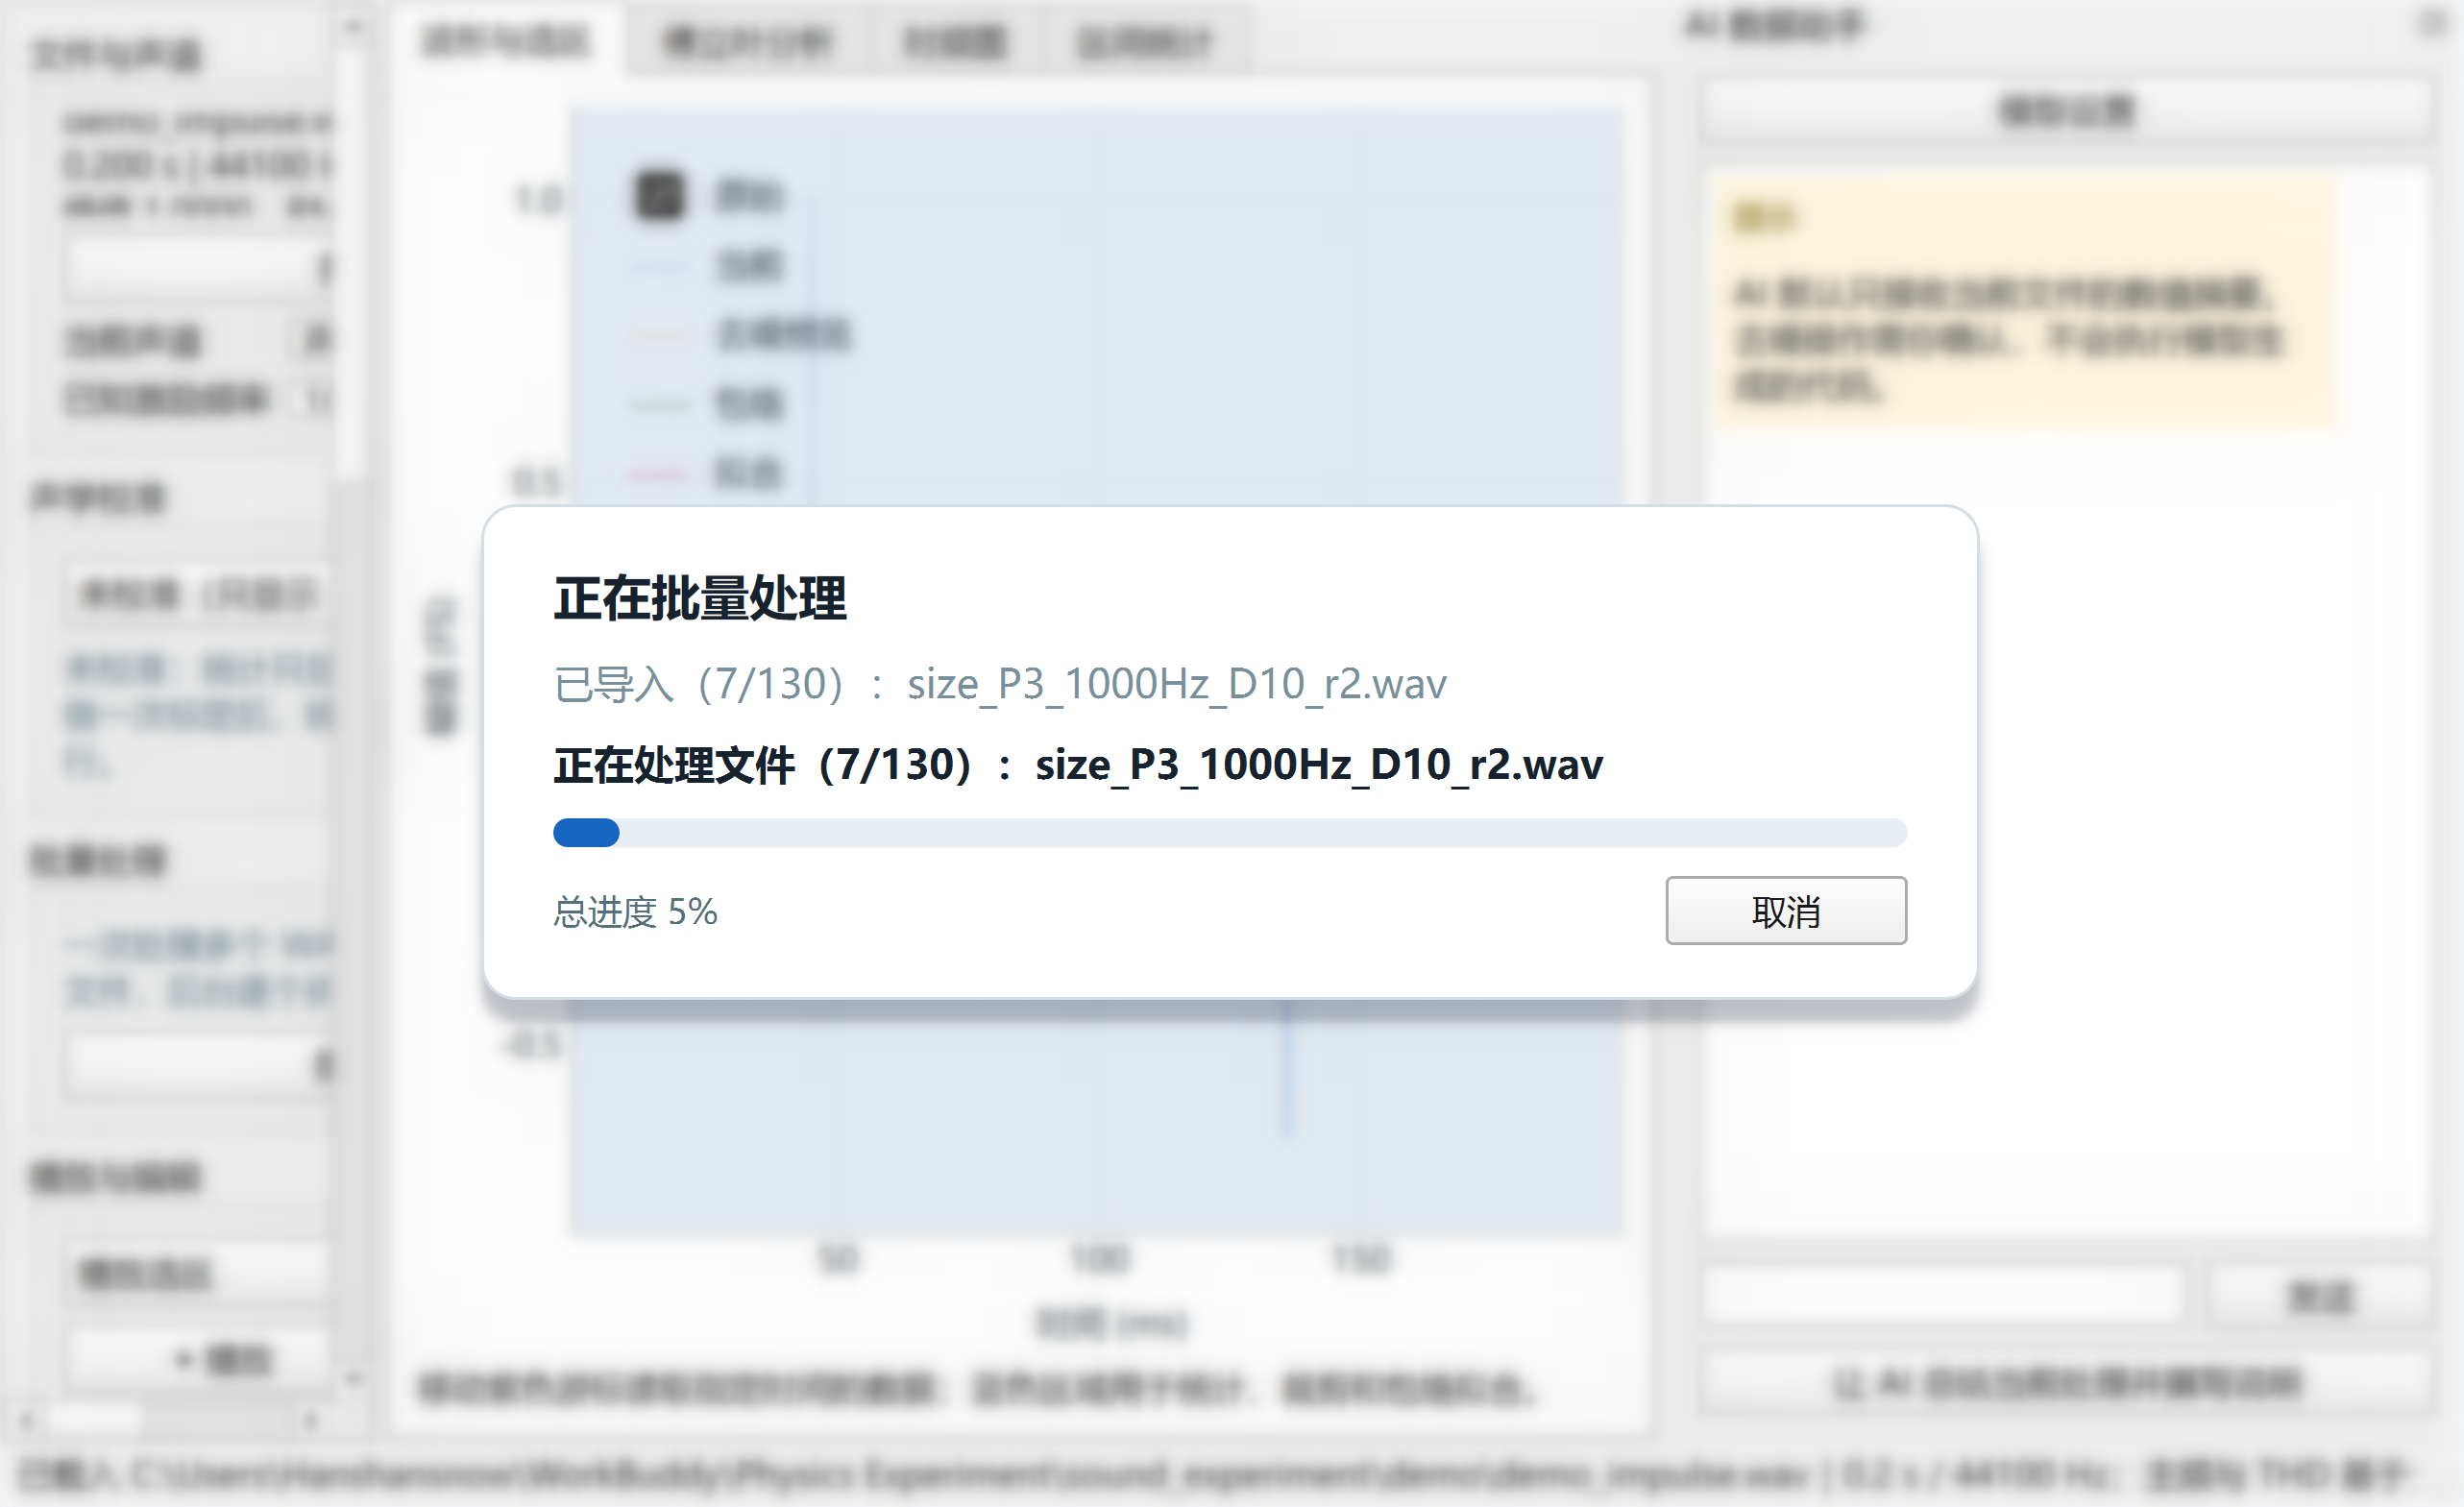
\includegraphics[width=0.86\textwidth]{10_batch_progress.png}
\caption{批处理进度遮罩。背景是主窗口的模糊快照，卡片同时显示当前文件与总进度。}
\label{fig:batch_progress}
\end{figure}

卡片上有三行信息：第一行“已导入（m/n）：文件名”表示第 m 个文件已读入内存；第二行“正在处理文件（m/n）：文件名”；下面是总进度条与百分比。两个数字分开显示，是因为读取大文件本身就要几秒，用户需要知道时间花在读盘还是算上。

\textbf{取消只在文件之间生效}。点“取消”后，当前文件会完整处理完再停，不会留下导出了一半的 TXT 或 PNG；已完成的文件保持原样，汇总文件正常收尾。

处理结束后弹窗给出汇总：共几个文件、成功几个、失败几个、用时多少秒、输出几个文件。有失败时列出前八个失败文件名与原因。

\subsection{脚本的保存与复用}

“保存脚本…”把当前步骤写成 JSON，“载入脚本…”读回来。脚本文件只含步骤和参数，不含文件列表，因此同一套流程可以反复用于不同批次。

关闭窗口时程序也会记住这次的步骤与输出目录，下次打开自动恢复，适合连续几天重复同一套处理。若想从空白开始，把步骤逐个删除即可。

\subsection{一个完整的例子}

以开孔透射实验为例，一百四十多个 WAV，文件名形如 \texttt{size\_\allowbreak P3\_\allowbreak 1000Hz\_\allowbreak D10\_\allowbreak r1.wav}。脚本可以配成四步：

\begin{enumerate}
  \item 冲击去噪：稳健阈值 8.0，最长修复 3\,ms，处理范围选全部声道；
  \item 区间统计：统计区间选“去掉首尾”，各 0.2\,s；已知激励频率选“文件名里的频率”；
  \item 导出统计 CSV：合并为一个文件，命名 \texttt{batch\_stats.csv}；
  \item 导出分析 TXT：合并为一个文件，章节里取消“原坐标”。
\end{enumerate}

跑完打开 CSV，先看“主频 (Hz)”这一列是不是每个文件都等于它标称的频率。有一个对不上，多半是那个文件名漏了 \texttt{Hz}，改名后单独重跑即可。这一步是命名与解析的唯一可靠校验，值得每次都做。

真正的隔声量要用基准文件与测试文件相减得到：同一频率、同一距离下，用密封基准板的主频电平减去测试板的主频电平即得 $\Delta L$，再按 $\tau = 10^{-\Delta L/10}$ 换算透射系数。批量只负责把每个文件的电平算准、排整齐，配对相减交给表格软件，这样每一步都能回溯到具体文件。

% ==================== 第 17 章 ====================
\section{推荐实验流程}


建议按以下流程处理每份实验录音：

\begin{enumerate}
  \item 导入 WAV，查看文件信息和削顶警告。
  \item 观察波形和时频图，初步判断是否存在冲击或异常区间。
  \item 运行傅立叶分析，记录主频、峰值振幅和 THD。
  \item 框选稳态区间并计算统计量；需要试听时播放选区，只关心某段响应时可先裁剪再重算。
  \item 检测冲击，预览后应用合适的修复或排除。
  \item 提取包络并拟合方程。
  \item 双通道实验再执行时延与电平分析。
  \item 导出处理后 WAV、分析数据 TXT、图像 PNG、统计 CSV 和数据处理报告。
  \item 文件较多时改用批量处理：先配好步骤脚本整批跑出统计 CSV，再挑代表文件单独出图。
  \item 将最终结论与原始录音、处理参数和图表一并存档。
\end{enumerate}

每一步的结论都应能回溯到对应的原始数据和算法参数。报告中应区分“直接测得”“算法估计”和“经校准换算”三类数据。

% ==================== 第 18 章 ====================
\section{常见错误与处理}

程序把所有异常都以弹窗形式报告，格式为“异常类型：具体消息”。例如文件被别的程序占用时，弹窗开头是 \texttt{PermissionError}，后面跟一句“另一个程序正在使用此文件”（\texttt{WinError 32}）。排查时请把这两部分一起记下来，再对照下表定位。

{\small
\begin{longtable}{@{}>{\raggedright\arraybackslash}p{0.24\textwidth}>{\raggedright\arraybackslash}p{0.30\textwidth}>{\raggedright\arraybackslash}p{0.40\textwidth}@{}}
\caption{常见错误、原因与处理办法}\\
\toprule
现象或提示 & 可能原因 & 处理办法 \\
\midrule
\endfirsthead
\toprule
现象或提示 & 可能原因 & 处理办法 \\
\midrule
\endhead
\bottomrule
\endfoot
双击启动脚本无反应、窗口一闪而过 & 依赖未安装、Python 解释器路径改变 & 打开命令行手动运行 \texttt{run\_app.bat}，按报错信息处理；必要时重新执行第 2 章的依赖安装 \\
提示缺少模块（如 \texttt{keyring}、\texttt{sounddevice}、\texttt{matplotlib}） & 依赖不完整（换机器或换环境后常见） & 在程序目录执行 \texttt{pip install -r requirements.txt}；打包版请改用 EXE，不要解压后移动内部文件 \\
提示“WAV 文件不存在” & 文件被移动、改名，或路径过长、含生僻字符 & 把文件复制到较短的英文路径（如 \texttt{D:\textbackslash data}）后重新打开 \\
提示“音频数据必须是非空的 [采样点, 声道] 数组” & 选到了只有文件头的空 WAV，或文件已损坏 & 用 Audacity 打开确认能播放，再“导出为 WAV（PCM）”重新生成 \\
打开后波形是一条直线 / 统计量全为 0 & 文件近乎静音，或实际不是所选声道 & 切换“当前声道”；检查录制增益与设备连接 \\
大文件点击“检测并预览”后界面变灰、遮罩在转 & 正常现象：计算在后台线程进行 & 等待遮罩消失即可；遮罩期间刻意禁用鼠标，避免数据竞争，不要反复点击 \\
Windows 标题栏显示“未响应”，但遮罩仍在转 & 主线程在等待底层计算或重绘，属短暂停顿 & 继续等待（大文件数秒）；若超过 1 分钟完全无变化，再按“闪退”处理 \\
程序直接消失（闪退） & 内存不足（数千万点文件）、或关闭窗口时后台任务未结束 & 先裁剪选区再分析；关闭其它占内存程序；退出前等遮罩消失；命令行启动可见具体异常 \\
提示“冲击检测至少需要 9 个采样点和正采样率” & 选区太短 & 扩大蓝色选区后重新检测 \\
提示“冲击检测输入包含 NaN 或无穷值” & WAV 中含非法采样值 & 用 Audacity 检查并重新导出；不要用二进制编辑器手工修补 \\
提示“区间内有效采样点不足” & 选区几乎全部被排除段覆盖 & 降低“最长修复”以外的排除范围，或提高阈值重新检测；也可缩小选区避开冲击段 \\
提示“统计区间无效：需要 $0 \leq \text{start}$ 且 $\text{start} < \text{end}$” & 选区起止颠倒或宽度为 0 & 重新拖选蓝色选区，确保左边界小于右边界 \\
“应用预览”按钮始终为灰色 & 还没有有效预览，或刚点过“关闭预览” & 先“检测并预览”；关闭预览后需重新检测才能应用 \\
“撤销上次处理”没反应 & 撤销栈为空，或已达上限（4 级 / 约 1.2 GB） & 无法再撤销；重要结果请先“导出处理后 WAV”或写回源文件 \\
写回源文件提示 \texttt{PermissionError} / 拒绝访问 & 文件被播放器、网盘同步、杀毒软件占用，或设为只读 & 关闭占用程序、取消只读属性后重试；也可用“导出处理后 WAV”另存到新文件 \\
写回后想恢复原始录音 & 程序已在同目录生成 \texttt{.bak-时间戳.wav} 备份 & 把备份文件改回原文件名即可还原 \\
点击播放没有声音 & 无可用输出设备、系统静音、设备被独占，或设备不支持该采样率 & 换输出设备、解除独占模式；程序会尝试重采样，仍失败则会提示“当前系统没有可用的音频输出设备” \\
AI 返回 401 / 403 & API Key 错误、无该模型权限或账户欠费 & 重新粘贴 Key；到厂商控制台确认余额与权限；注意不要多复制空格 \\
AI 返回 404 或 model not found & Base URL 少了（或多了）\texttt{/v1}，或模型名不存在 & 直接改用厂商预设；自定义时用浏览器访问 \texttt{Base URL/models} 确认返回 JSON \\
AI 返回 429 & 触发限流或配额用尽 & 降低请求频率，稍后重试；检查套餐额度 \\
AI 请求超时 & 网络慢、代理不稳定，或上下文过长 & 默认已是 120 s，仍超时就调到 300 s；换网络或关闭代理后重试 \\
AI 提示“模型响应缺少 choices[0].message” & 返回内容不是 OpenAI 兼容格式（常见于网关错误页或中转服务） & 用 \texttt{curl} 或浏览器直接请求该地址，确认返回标准 JSON；换用官方地址 \\
导出的 CSV 在 Excel 里中文乱码 & 双击打开时未按 UTF-8 解析 & 程序按 UTF-8（带 BOM）写入；如仍异常，用 Excel 的“数据→从文本/CSV”并手动选择 UTF-8 \\
生成 HTML 报告失败 & 缺少 matplotlib & \texttt{pip install matplotlib}；打包版请用分发版 EXE \\
界面中文显示为方块 & 系统缺少中文字体 & 安装微软雅黑与宋体；服务器/精简系统尤其常见 \\
\end{longtable}
}

\begin{itemize}
  \item 遇到无法判断的问题时，优先在命令行启动程序，异常会完整打印在控制台，比弹窗信息更详细。
  \item 处理实验数据前请先备份原始 WAV。程序的自动备份与撤销只能覆盖操作失误，不能替代备份。
  \item AI 不可用不影响任何本地功能：去噪、统计、包络、傅立叶与报告生成都只依赖本地算法。
\end{itemize}

\section{常见问题}

\subsection{无法打开文件}

确认文件扩展名为 \texttt{.wav}，且不是损坏或受保护的文件。程序支持单声道和双声道 WAV。若文件由其他设备生成，建议先确认其编码格式为 PCM。

\subsection{频谱看不到目标频率}

检查“已知激励频率”是否填写正确，并切换频率轴刻度或调整显示范围。若录制时信号本身过弱、削顶或混入了强噪声，频谱峰值可能不清楚。此时应先从波形和时频图判断信号质量，而不是盲目调整频谱参数。

\subsection{去噪误标记正常波峰}

提高“稳健阈值”，缩短“最长修复”，并重新预览。若正常信号仍被频繁标记，应先检查数据是否削顶、直流偏置过大或存在持续脉冲序列。必要时放弃自动去噪，手动框选有效区间进行统计。

\subsection{AI 连接失败}

检查 Base URL、模型名称、API Key、网络和超时设置。不要把 Key 写入报告、代码或聊天内容。AI 不可用时，程序的手动分析、去噪、统计和导出功能不受影响。

% ==================== 第 19 章 ====================
\section{安全与数据管理}

\begin{itemize}
  \item 原始实验录音应备份，不要把处理后的文件覆盖原始数据。
  \item API Key 仅保存在本机钥匙串或临时输入，不应提交到代码仓库。
  \item 上传给 AI 的默认内容是数值摘要和工具结果，不是完整 WAV；使用外部模型服务时应遵守平台隐私和数据管理要求。
  \item 报告中应区分“直接测得”“算法估计”和“经校准换算”的数据。
  \item dBFS 不等于 dB SPL。只有完成声学校准后，才能输出真实声压级。
\end{itemize}

% ==================== 附录 ====================
\newpage
\appendix

\section{参数速查表}

\begin{table}[htbp]
\centering
\caption{常用参数默认值}
\begin{tabular}{@{}lll@{}}
\toprule
参数 & 默认值 & 说明 \\
\midrule
已知激励频率 & 1000 Hz & 设为 0 时自动估计 \\
稳健阈值 & 8.0 & 越大检出越少 \\
最长修复 & 3.0 ms & 短于该值才插值修复 \\
频谱幅值刻度 & Linear (AMP) & 可切换 dBFS \\
频率轴刻度 & 线性 & 可切换对数 \\
包络模型 & auto & 可选常数、线性、指数 \\
图像版式 & 论文单栏 & 可选论文双栏、屏幕像素 \\
图像分辨率 & 600 dpi & 仅论文版式 \\
图例位置 & 坐标区外（图底） & 可改坐标区内或不显示 \\
TXT 坐标取法 & 每秒 1000 点 & 可改步长抽稀或全部采样点 \\
TXT 大表阈值 & 500 万行 & 超过时导出前二次确认 \\
批量稳健阈值 & 8.0 & 与单文件去噪同一算法 \\
批量统计区间 & 全文件 & 可改去掉首尾或固定区间 \\
批量 CSV 输出 & 合并为一个 & 一行一个文件，含 21 项统计量 \\
校准偏移 K & 由参数推算 & 也可用已知声压级标定，二者等效 \\
满幅输入电压 & 1.0 Vrms & 声卡最不确定的参数，有条件改用标定 \\
AI 请求超时 & 120 s & 可调 5--600 s，连接阶段 15 s \\
AI 回答渲染 & Markdown & 标题、列表、表格、代码与链接\\
\bottomrule
\end{tabular}
\end{table}

\section{文件清单}

\begin{table}[htbp]
\centering
\caption{主要文件与目录（安装位置：\texttt{D:\textbackslash WAV\_Analyzer}）}
\begin{tabular}{@{}>{\raggedright\arraybackslash}p{3.9cm}>{\raggedright\arraybackslash}p{10.1cm}@{}}
\toprule
路径 & 说明 \\
\midrule
\texttt{run\_app.bat} & Windows 启动脚本 \\
\texttt{run\_app.py} & Python 启动入口 \\
\texttt{app/} & 桌面界面模块（含 \texttt{txt\_export\_dialog.py} 导出设置、\texttt{batch\_dialog.py} 批量脚本编辑、\texttt{batch\_progress.py} 进度遮罩、\texttt{chat\_view.py} 会话气泡、\texttt{markdown\_lite.py} 轻量 Markdown 渲染） \\
\texttt{core/} & 信号处理核心算法（含 \texttt{txt\_export.py} 文本导出排版、\texttt{batch.py} 批量流水线引擎、\texttt{calibration.py} 声压级换算） \\
\texttt{ai/} & AI 助手与工具调用 \\
\texttt{tests/} & 自动化测试（121 项，含批量流水线、会话气泡与 Markdown 渲染） \\
\texttt{demo/} & 合成演示数据与报告样例 \\
\texttt{docs/} & 使用说明书与配图 \\
\texttt{requirements.txt} & 依赖包列表 \\
\texttt{wav\_analyzer.ico} & 程序图标（桌面快捷方式绑定此图标） \\
\texttt{WAV\_Analyzer.spec} & PyInstaller 打包配置（重建单文件 EXE 用） \\
\bottomrule
\end{tabular}
\end{table}

\section{版本说明}

本手册对应程序 1.5 版，安装位置为 \texttt{D:\textbackslash WAV\_Analyzer}，桌面已创建“WAV Analyzer”快捷方式。自动化测试共 141 项全部通过，覆盖核心算法、界面交互、大文件处理流水线、批量流水线、声学校准、图像导出、文本导出与报告导出。自动去噪阈值已通过合成信号验证，但应用到真实实验数据时仍应结合波形、频谱和时频图复核。

\begin{itemize}
  \item \textbf{1.4}：AI 助手改进——提问与回答改用不同底色的气泡并区分提示与错误，回答按 Markdown 渲染（标题、列表、表格、代码、链接）；去掉“是否用钥匙串保存 Key”的勾选框，改为固定用 Windows 钥匙串保存并声明不向任何人透露 Key；默认超时改为 120 s 并给超时、连接、鉴权失败分别给出提示；AI 去噪确认改为只问一次、0 段不再弹窗。
  \item \textbf{1.5}：新增声学校准——按灵敏度/前置增益/满幅电压推算偏移 $K$，或用已知声压级标定；统计、CSV、TXT、HTML 报告与批量处理同步输出 dB SPL；未校准时不出声压级，避免给出无依据的数。
  \item \textbf{1.3}：新增批量处理——可保存的步骤脚本、多选文件只记路径、独立线程执行、主窗口模糊遮罩与逐文件进度、取消只在文件之间生效；TXT 与 CSV 支持“合并为一个文件”；修正步骤摘要把合并文件名也写成“后缀 xxx”的问题，长摘要改为折行显示。
  \item \textbf{1.2}：新增导出分析 TXT，七段结构、定宽 ASCII 对齐、坐标取法三选项、区间统计多选，并附源 WAV 的 MD5 指纹；图像导出新增论文版式（单栏 3.50$\times$2.45\,in、双栏 7.00$\times$2.60\,in、600 dpi、刻度朝内四边齐全、次刻度），图例统一移到坐标区外图底一行，包络与拟合在论文版式下自动拆为上下双图，包络线绘图时做 5\,ms 平滑；修复导出对话框默认版式与深色背景冲突的问题。
  \item \textbf{1.1}：新增裁剪、播放试听与应用更改到源文件；新增导出图像 PNG（波形、频谱、时频图，中文宋体 + 西文 Times New Roman 制图规范）；区间统计改为中文名、数值、含义三列；冲击检测改为分块计算，长音频不再出现假死与闪退，并增加处理进度提示；模型设置提供 DeepSeek、Moonshot、OpenAI 预设；手册新增“常见错误与处理”一章。
  \item \textbf{1.0}：首个可用版本，具备去噪、傅立叶分析、时频分析、包络拟合、区间统计、双通道分析、AI 助手与报告导出。
\end{itemize}

\end{document}
